%%%%%%%%%%%%%%%%%%%%%%%%%%%%%%%%%%%%%%%%%
% Beamer Presentation
% LaTeX Template
% Version 1.0 (10/11/12)
%
% This template has been downloaded from:
% http://www.LaTeXTemplates.com
%
% License:
% CC BY-NC-SA 3.0 (http://creativecommons.org/licenses/by-nc-sa/3.0/)
%
%%%%%%%%%%%%%%%%%%%%%%%%%%%%%%%%%%%%%%%%%
\documentclass[smaller,handouts]{beamer}

%----------------------------------------------------------------------------------------
%	PACKAGES AND THEMES
%----------------------------------------------------------------------------------------
\mode<handout>{
  \usepackage{pgf}
  \usepackage{pgfpages}

\pgfpagesdeclarelayout{4 on 1 boxed}
{
  \edef\pgfpageoptionheight{\the\paperheight} 
  \edef\pgfpageoptionwidth{\the\paperwidth}
  \edef\pgfpageoptionborder{0pt}
}
{
  \pgfpagesphysicalpageoptions
  {%
    logical pages=4,%
    physical height=\pgfpageoptionheight,%
    physical width=\pgfpageoptionwidth%
  }
  \pgfpageslogicalpageoptions{1}
  {%
    border code=\pgfsetlinewidth{2pt}\pgfstroke,%
    border shrink=\pgfpageoptionborder,%
    resized width=.5\pgfphysicalwidth,%
    resized height=.5\pgfphysicalheight,%
    center=\pgfpoint{.25\pgfphysicalwidth}{.75\pgfphysicalheight}%
  }%
  \pgfpageslogicalpageoptions{2}
  {%
    border code=\pgfsetlinewidth{2pt}\pgfstroke,%
    border shrink=\pgfpageoptionborder,%
    resized width=.5\pgfphysicalwidth,%
    resized height=.5\pgfphysicalheight,%
    center=\pgfpoint{.75\pgfphysicalwidth}{.75\pgfphysicalheight}%
  }%
  \pgfpageslogicalpageoptions{3}
  {%
    border code=\pgfsetlinewidth{2pt}\pgfstroke,%
    border shrink=\pgfpageoptionborder,%
    resized width=.5\pgfphysicalwidth,%
    resized height=.5\pgfphysicalheight,%
    center=\pgfpoint{.25\pgfphysicalwidth}{.25\pgfphysicalheight}%
  }%
  \pgfpageslogicalpageoptions{4}
  {%
    border code=\pgfsetlinewidth{2pt}\pgfstroke,%
    border shrink=\pgfpageoptionborder,%
    resized width=.5\pgfphysicalwidth,%
    resized height=.5\pgfphysicalheight,%
    center=\pgfpoint{.75\pgfphysicalwidth}{.25\pgfphysicalheight}%
  }%
}


  \pgfpagesuselayout{4 on 1 boxed}[a4paper, border shrink=5mm, landscape]
  \nofiles
}


\usepackage{algorithm,algorithmic}
\usepackage{graphicx} % Allows including images
\usepackage{booktabs} % Allows the use of \toprule, \midrule and \bottomrule in tables
\usepackage{tikz}
\usepackage{color}
\usepackage{tkz-graph}
\usepackage[utf8]{inputenc}
\usepackage[danish]{babel}
\usepackage{mathtools}% Loads amsmath
\usepackage{amsmath}
% \usepackage{graphicx}
% \usepackage[caption=false]{subfig}
% \usepackage{braket}
% \usepackage{geometry}
% \usepackage{empheq}
\usepackage{amssymb}

%\definecolor{kugreen}{RGB}{50,93,61}
%\setbeamercovered{transparent=20}


\mode<presentation> {
% \useoutertheme{sidebar}
% infolines
% miniframes
% shadow
% sidebar
% smoothbars
% smoothtree
% split
% tree

% \useinnertheme{rounded}
% rectangles
% circles
% inmargin
% rounded
 \setbeamercolor{alerted text}{fg=blue}
% \setbeamercolor{background canvas}{bg=white}
% \setbeamercolor{block body alerted}{bg=normal text.bg!90!green}
% \setbeamercolor{block body}{bg=normal text.bg!90!green}
% \setbeamercolor{block body example}{bg=normal text.bg!90!green}
% \setbeamercolor{block title alerted}{use={normal text,alerted text},fg=alerted text.fg!75!normal text.fg,bg=normal 
% text.bg!75!black}
% \setbeamercolor{block title}{bg=blue}
% \setbeamercolor{block title example}{use={normal text,example text},fg=example text.fg!75!normal text.fg,bg=normal 
% text.bg!75!green}
% \setbeamercolor{fine separation line}{}
% \setbeamercolor{frametitle}{fg=white}
% \setbeamercolor{item projected}{fg=black}
% \setbeamercolor{normal text}{bg=black,fg=black}
% \setbeamercolor{palette sidebar primary}{use=normal text,fg=normal text.fg}
% \setbeamercolor{palette sidebar quaternary}{use=structure,fg=structure.fg}
% \setbeamercolor{palette sidebar secondary}{use=structure,fg=structure.fg}
% \setbeamercolor{palette sidebar tertiary}{use=normal text,fg=normal text.fg}
% \setbeamercolor{section in sidebar}{fg=brown}
% \setbeamercolor{section in sidebar shaded}{fg=grey}
% \setbeamercolor{separation line}{}
% \setbeamercolor{sidebar}{bg=green}
% \setbeamercolor{sidebar}{parent=palette primary}
% \setbeamercolor{structure}{bg=black, fg=green}
% \setbeamercolor{subsection in sidebar}{fg=brown}
% \setbeamercolor{subsection in sidebar shaded}{fg=grey}
% \setbeamercolor{title}{fg=brown}
% \setbeamercolor{titlelike}{fg=brown}
\setbeamertemplate{blocks}[rounded][shadow=true]


%  \usetheme{PaloAlto}
 % \usecolortheme[named=kugreen]{structure}
 % \useinnertheme{circles}
 % \usefonttheme[onlymath]{serif}
 % \setbeamercovered{transparent}
 % \setbeamertemplate{blocks}[rounded][shadow=true]

% The Beamer class comes with a number of default slide themes
% which change the colors and layouts of slides. Below this is a list
% of all the themes, uncomment each in turn to see what they look like.

%\usetheme{default}
%\usetheme{AnnArbor}
\usetheme{Antibes}
%\usetheme{Bergen}
%\usetheme{Berkeley}
%\usetheme{Berlin}
%\usetheme{Boadilla}
%\usetheme{CambridgeUS}
%\usetheme{Copenhagen}
%\usetheme{Darmstadt}
%\usetheme{Dresden}
%\usetheme{Frankfurt}
%\usetheme{Goettingen}
%\usetheme{Hannover}
%\usetheme{Ilmenau}
%\usetheme{JuanLesPins}
%\usetheme{Luebeck}
%\usetheme{Madrid}
%\usetheme{Malmoe}
%\usetheme{Marburg}
%\usetheme{Montpellier}
%\usetheme[width=50pt]{PaloAlto}
%\usetheme{Pittsburgh}
%\usetheme{Rochester}
%\usetheme{Singapore}
%\usetheme{Szeged}
%\usetheme{Warsaw}

% As well as themes, the Beamer class has a number of color themes
% for any slide theme. Uncomment each of these in turn to see how it
% changes the colors of your current slide theme.

%\usecolortheme{albatross}
%\usecolortheme{beaver}
%\usecolortheme{beetle}
%\usecolortheme{crane}
%\usecolortheme{dolphin}
%\usecolortheme{dove}
%\usecolortheme{fly}
%\usecolortheme{lily}
%\usecolortheme{orchid}
%\usecolortheme{rose}
%\usecolortheme{seagull}
%\usecolortheme{seahorse}
%\usecolortheme{whale}
%\usecolortheme{wolverine}
\usecolortheme[rgb={0,0.4,0}]{structure}

%\setbeamertemplate{footline}[frame number]
%\setbeamertemplate{footline} % To remove the footer line in all slides uncomment this line
%\setbeamertemplate{footline}[page number] % To replace the footer line in all slides with a simple
%slide count uncomment this line


\setbeamertemplate{navigation symbols}{} % To remove the navigation symbols from the bottom of all
%slides uncomment this line
}
%\expandafter\def\expandafter\insertshorttitle\expandafter{%
 % \insertshorttitle\hfill%
 % \insertframenumber\,/\,\inserttotalframenumber}

\addtobeamertemplate{navigation symbols}{}{%
    \usebeamerfont{footline}%
    \usebeamercolor[fg]{footline}%
    \hspace{1em}%
    Slide \insertframenumber
}
\setbeamercolor{footline}{fg=black}
\setbeamerfont{footline}{series=\bfseries}

 
 
\usetikzlibrary{decorations.pathreplacing}	

% \usetikzlibrary{arrows,decorations.pathmorphing,backgrounds,positioning,fit,matrix} 
% \tikzstyle{vertex}=[circle,fill=black!25,minimum size=15pt,inner sep=0pt]
% \tikzstyle{selectedvertex} = [vertex, fill=red!24] 
% \tikzstyle{edge} = [draw,thick,-] 
% \tikzstyle{arc}= [draw,thick,->,shorten >=1pt,>=stealth'] 
% \tikzstyle{arcl} = [draw,thick,->,shorten>=1pt,>=stealth',bend left=25] 
% \tikzstyle{arcr} = [draw,thick,->,shorten >=1pt,>=stealth']
% \tikzstyle{rpath}=[draw, thick,->,shorten >=1pt,>=stealth',red, opacity=0.4]
% \tikzstyle{weight} = [font=\small] 
% \tikzstyle{selected edge} = [draw,line width=5pt,-,red!50]
% \tikzstyle{ignored edge} = [draw,line width=5pt,-,black!20] 
% \newcommand*{\vpointer}{\vcenter{\hbox{\scalebox{2}{\Huge\pointer}}}}	
% \def\Arrow{\raisebox{3\height}{\scalebox{3}{$\Rightarrow$}}}
\tikzstyle{arc}= [draw,thick,->,shorten >=2pt,>=stealth'] 
%\tikzstyle{vertex}=[circle,fill=black!25,minimum size=15pt,inner sep=0pt]
\tikzstyle{vertex}=[circle, draw, inner sep=0pt, minimum size=10pt]
\newcommand{\vertex}{\node[vertex]}
\def\Arrow{{\scalebox{2}{$\Rightarrow$}}}

%----------------------------------------------------------------------------------------
%	TITLE PAGE
%----------------------------------------------------------------------------------------

\title[]{Et lokalsøgningssystem til at løse diskrete 
optimeringsproblemer}% The short title appears at 
%the bottom of every slide, the full title is only on the title page

\author[]{Bo Stentebjerg-Hansen\\{ \scriptsize Vejleder: Marco Chiarandini}}
\institute[IMADA] 
% Your institution as it will appear on the bottom of every slide, may be
%shorthand %to save space
{
Syddansk Universitet \\ % Your institution for the title page
\medskip
Institut for Matematik og Datalogi
%\textit{IMADA} % Your email address
}

\date{3. marts 2016} % Date, can be changed to a custom date

\begin{document}

\begin{frame}
%\frametitle{Et lokalsøgningssystem til at løse diskrete 
%optimeringsproblemer}
\titlepage % Print the title page as the first slide

\end{frame}

\begin{frame}
\frametitle{Overblik} % Table of contents slide, comment this block out to remove it
\tableofcontents % Throughout your presentation, if you choose to use \section{} and \subsection{}
%commands, these will automatically be printed on this slide as an overview of your presentation
\end{frame}

%----------------------------------------------------------------------------------------
%	PRESENTATION SLIDES
%----------------------------------------------------------------------------------------

%------------------------------------------------
\section{Introduktion} % Sections can be created in order to organize your presentation into
%discrete blocks, all sections and subsections are automatically printed in the table of contents as
%an overview of the talk
%------------------------------------------------
%\subsection{Subsection Example} % A subsection can be created just before a set of slides with a
%common theme to further break down your presentation into chunks

\begin{frame}
\frametitle{Diskrete optimeringsproblemer}
\begin{columns}[T]
    \begin{column}[T]{.5\textwidth}
        \vspace{0pt}
\onslide<1->   En diskret optimeringsproblem $p$ består af: 
\pause
    \begin{itemize}[<+->]
\item $n$ variable \textbf{x}, $\mathbf{x} \in \mathbb{Z}^n$
\item $m$ betingelser \textbf{C}
\item Evaluerings funktion $f(x)$ \medskip \\
\end{itemize}
 \onslide<5-> \alert{\[min \{\; f(x) \;| \; x  \in feas(p)\}\]} \\
 \onslide<6-> Kan være NP-hårde problemer
 \end{column}
    \hfill
    \begin{column}[T]{.5\textwidth}
      \onslide<6->{Eksempel: Skemalægningsinstans}
      \pause \pause
\begin{itemize}[<+->]
 \item Variable: Klasser der skal skemalægges
 \item Betingelser: Ingen overlap, krav til lokaler, tidspunkter, osv
\item Evaluering: Totale antal af mellemtimer
 \item Bedste løsning: Den løsning som overholder alle betingelser og giver færrest mellemtimer
\end{itemize}
    \end{column}
    \end{columns}
\end{frame}

\begin{frame}
 \frametitle{Løsningsmetoder}
%  \begin{columns}[T]
%  \begin{column}[T]{.5\textwidth} \vfill
  - Algoritmer til specifikke problemer  \\ \hspace{1cm}\pause
      - Approximations algoritmer \\  \hspace{1cm}\pause 
      - Dynamisk programmering \\ \pause
 - \dots \\ 
 - Satisfiability encoding \\ \pause 
 - Lineær heltalsprogramming \\ \pause 
 - Constraint Programming \\ \pause
 - Lokalsøgning \\ 
 - \dots
%  \end{column} 
%  \onslide<1->
% \begin{column}[T]{.5\textwidth} \vfill
%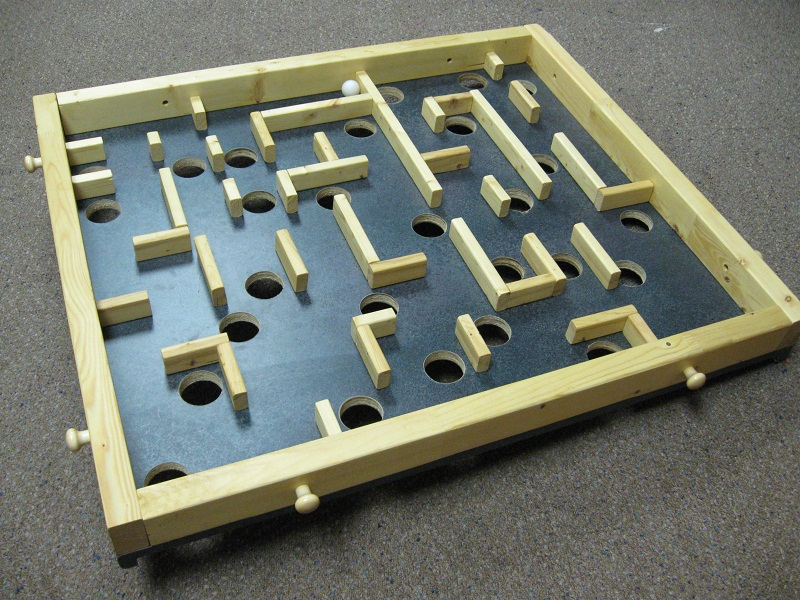
\includegraphics[scale=0.45]{lokals3.jpg}
% 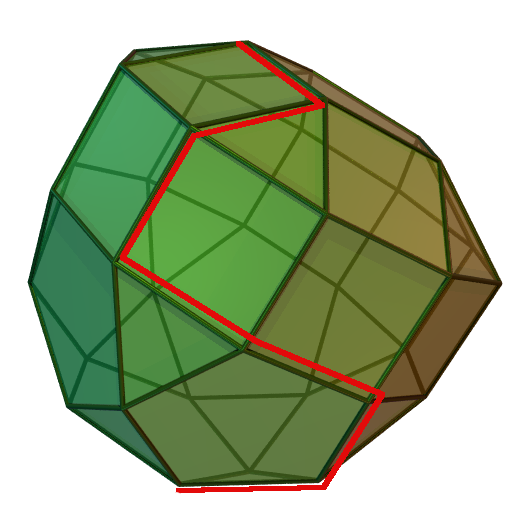
\includegraphics[scale=0.2]{lokals6.png}
% \end{column}
% \end{columns}
 
\end{frame}

%--------------------------------------------------

\begin{frame}
\frametitle{Lineær helttalsprogrammering}
\begin{itemize}[<+->]  
% \item Revised simplex metode, .
\item Model baseret på uligheder
\end{itemize}
\begin{table}[]
\begin{center}
\label{my-label}
\begin{tabular}{llrcrlrl}
Minimize   & z =&$2x_1$        & +  & $x_2$       & + & $x_3$ &          \\
subject to &     &$-x_1$        & + & $2x_2$      &   &       & $\leq 1$  \\
           &     &$x_1$         & + & $x_2$       & + & $x_3$ & $=2$     
               
\end{tabular}
\end{center}
$\qquad \qquad $ $x_1,x_2,x_3 $  $\in$ $\mathbb{Z}^+$ 
\end{table}

\begin{itemize}[<+->]
\item Gurobi, CPLEX, SCIP, GLPK
\item \alert{Kan ikke altid finde en (optimal) løsning inden for rimelig tid}
\item Kan garantere at en løsning er optimal 
\end{itemize}

    
\end{frame}


%-----------------------------------------------------

\begin{frame}
\frametitle{Constraint Programming (CP)}
\begin{columns}[T]
    \begin{column}[T]{.52\textwidth}
    \vspace{0.1cm}
    \begin{itemize}[<+->]
\item Bruger søgetræer + propagation til at finde en løsning
\item Mere naturlig formulering af problemer
\item Flere muligheder for at modeller et problem
\item \alert{Men mindre egnet til optimeringsproblemer}
\item Fx Gecode, CHIP, Prolog, \dots
\end{itemize}
\end{column} 
\begin{column}[T]{.5\textwidth} \vfill
\begin{center}
4-Queens problem \\
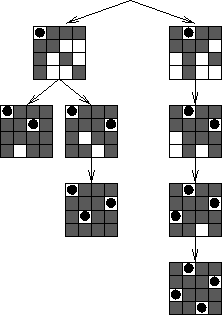
\includegraphics[scale=0.5]{cp.png}
\end{center}
\end{column}
\end{columns}
\end{frame}
%-----------------------------------------------------

\begin{frame}
\frametitle{Lokalsøgning}
\begin{columns}[T]
    \begin{column}[T]{.5\textwidth}\begin{itemize}[<+->]
\item ``Trial and error'' teknik
\item Alle variable skal have en værdi først
\item Delt op implicitte og bløde betingelser
\item Ændre få variable ad gangen og beregner effekten
\item \alert{Kan ikke garantere optimalitet}
\item Ofte implementeret forfra til specifikke problemer
\item Genenral Purpose lokalsøgningssystemer
\end{itemize}
\end{column} 
\begin{column}[T]{.5\textwidth} \vfill
%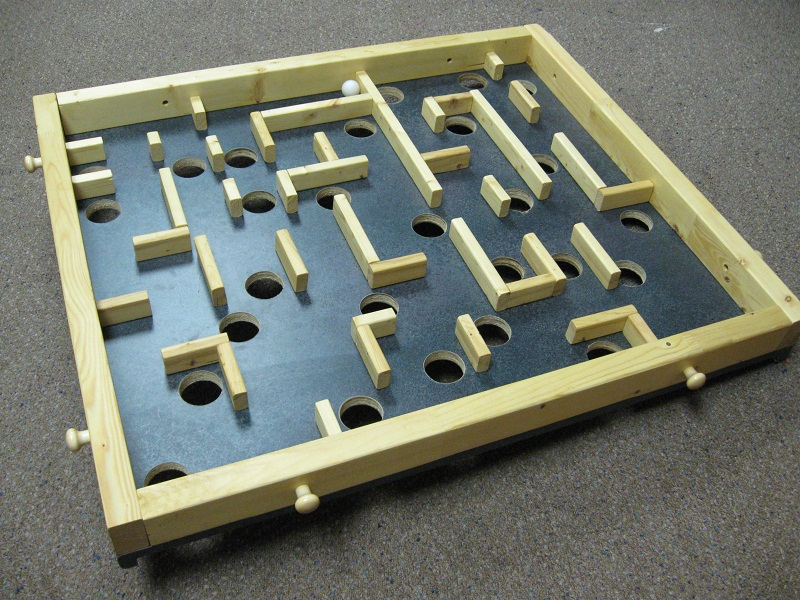
\includegraphics[scale=0.45]{lokals3.jpg}
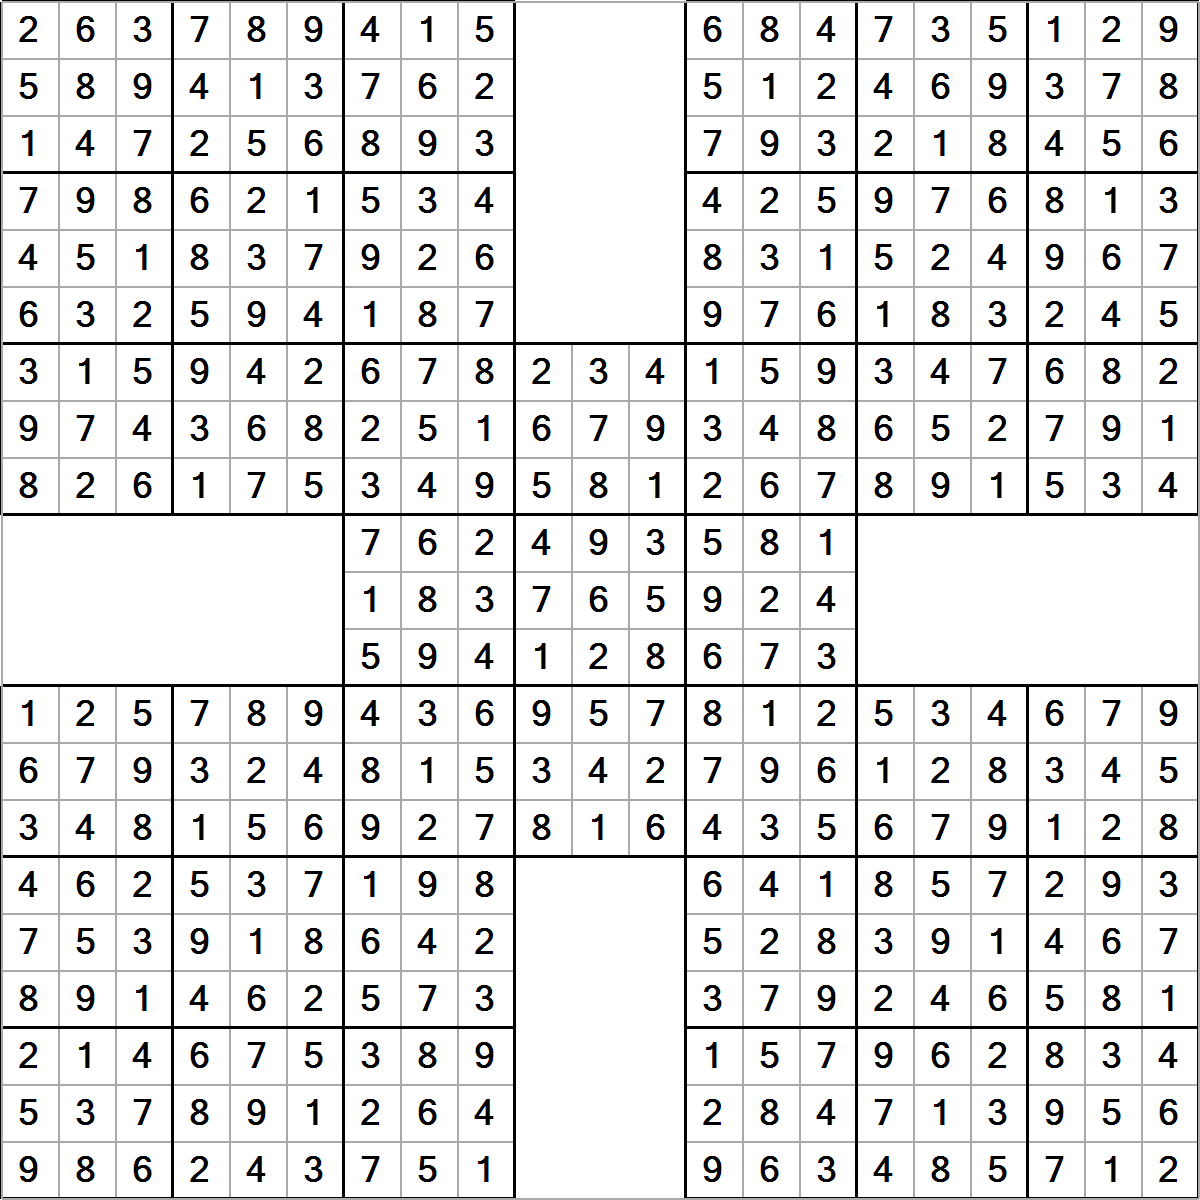
\includegraphics[scale=0.2]{lokals5.png}
\end{column}
\end{columns}
\end{frame}

\begin{frame}
 \frametitle{General purpose lokalsøgningssystemer}
 \begin{columns}[T]
    \begin{column}[T]{.5\textwidth}
     \begin{enumerate}[<+->]
  \item EasyLocal++ {\scriptsize [L. Gaspero \& A. Schaerf]}
  \begin{itemize}[<+->]
   \item Lokalsøgningsalgoritmer implementeret
   \item Bruger definere hvilke der skal bruges 
   \item Hotspots skal implementeres af bruger
  \end{itemize}
     \item Comet {\scriptsize [Van Hentenryck \& Michel]}
  \begin{itemize}[<+->]
   \item Først betingelsesbaseret lokalsøgningssystem
   \item Mulighed for udvidelse
   \item Ikke længere vedligeholdt
  \end{itemize}
\end{enumerate}
\end{column} 
\begin{column}[T]{.5\textwidth}
     \begin{enumerate}[<+->]
     \setcounter{enumi}{2}
       \item LocalSolver {\scriptsize [Innovation 24]}
  \begin{itemize}[<+->]
   \item Matematisk modellering
   \item Lineær- og heltalsprogrammering
   \item Kommerciel Solver	
  \end{itemize}
\item OscaR  {\scriptsize [R. Landtsheer]}
  \begin{itemize}[<+->]
   \item Inspireret af Comet
   \item Forholdsvis nyt
  \end{itemize}
   \end{enumerate}  
\end{column}
\end{columns}
% \footnotetext[1]{http://www.localsolver.com/}
% \footnotetext[2]<5->{https://bitbucket.org/satt/easylocal-3}
% \footnotetext[3]<8->{Constrainted-Based Local Search, P. Hentenryck \& L. Michel}
% \footnotetext[4]<12->{http://oscarlib.bitbucket.org/cbls.html}
\end{frame}

% \begin{frame}
%  \frametitle{Hybridsystemer}
%  \begin{itemize}[<+->]
%   \item Kan de bedste elementer fra løsningsmetoderne kombineres?
%   \item Deklarativ programmering med lokalsøgning. 
%   \item Matematisk modellering eller Constraint Programming? 
%   \item Eksisterende hybridsystemer: Comet, LocalSolver og OscaR.
%  \end{itemize}
% \end{frame}

% \begin{frame}
%  \frametitle{Matematisk programmering med lokalsøgning}
%  \begin{minipage}{0.52\linewidth}
%  \begin{itemize}[<+->]
%   \item En bruger kan fokusere på modellen.
%   \item Kan anvende metoder fra heltalsprogrammering.
%   \item LocalSolver: Et effektivt, men kommercielt produkt.
%  \end{itemize}
%  \end{minipage} \hfill
%  \onslide<3>
%  \begin{minipage}{0.4\linewidth}
%   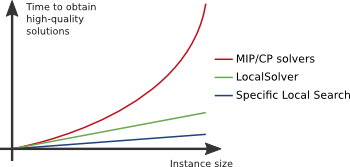
\includegraphics[scale=0.25]{localsolver.png}
%  \end{minipage}
% 
%  
%  \end{frame}
% 
% 
% \begin{frame}
%  \frametitle{Betingelsesbaseret lokalsøgning}
%  \begin{itemize}[<+->]
%   \item En bruger kan fokusere på modellen. 
%   \item Invarianter effektiviserer lokalsøgning.
%   \item Opbygger en graf til evaluering.
%   \item Comet: Første betingelsesbaseret lokalsøgningssystem.
%   \item OscaR: Inspireret af Comet, stadig under udvikling.
%  \end{itemize}
% \end{frame}


\begin{frame}
 \frametitle{Hvorfor et andet lokalsøgningssystem?}
 \begin{itemize}[<+->]
 \item Kombinerer CP og lokalsøgning på en ny måde: 
 \begin{itemize}[<+->]
%   \item[--] Ikke kun modelleringsmæssigt
  \item[--] Ikke som ``large scale neighborhood search'' {\scriptsize [P. Shaw] \footnotemark }
 \end{itemize}
 \item Undersøger effekten af (offline) CP domæne reducering og variable fiksering
 \item Bruger CP som konstruktions heuristik
 \item Tester effekten af envejsbetingelser
 \item \alert{Undersøger en ny evalueringsmetode i lokalsøgning}
  \begin{itemize}[<+->]
  \item[--] Leksikografisk vægtning
 \end{itemize}
 \end{itemize}
 \footnotetext[1]{\scriptsize Using constraint programming and 
local search methods to solve vehicle
routing problems}
\end{frame}


\section{Lokalsøgnings elementer}
% 
% \begin{frame}
%  \frametitle{Invarianter, envejsbetingelser og bløde betingelser}
%  \begin{itemize}[<+->]
%   \item 
%  \end{itemize}
%  
% \end{frame}
% 


\begin{frame}
 \frametitle{Begreber i lokalsøgning}
  \begin{columns}[T]
   \begin{column}[T]{.5\textwidth}
   Modellering: 
   \pause
 \begin{itemize}[<+->]
 \item Variable:  search space $S(p)$, løsningsrepræsentation
 \item Betingelser: 
 \begin{itemize}[<+->]
  \item[--] Implicitte betingelser
  \item[--] Envejsbetingelser
  \item[--] Bløde betingelser
  
 \end{itemize}
\item Evaluerings funktion: kvaliteten af en løsning
%   \item Search space $S(I)$: alle løsninger
%   \item Step funktion: hvordan går vi fra løsning $a$ til $b$ 
%   \item Neighborhood: løsninger tæt på en given løsning
%   \item Evaluerings funktion: kvaliteten af en løsning
%   \item Start løsning er krævet
%   \item Termineringskriterium: Hvornår skal søgningen stoppe
 \end{itemize}
  \end{column}
   \begin{column}[T]{.5\textwidth}
   \onslide<8->
   Søgning:
   \onslide<9->
    \begin{itemize}[<+->]
     \item (Konstruktions heuristik)
     \item Neighborhood \pause
     \item Lokalsøgning
     \item Metaheuristikker
      \begin{itemize}[<+->]
  \item[--] Tabu søgning
  \item[--] Iterativ lokalsøgning
  \item[--] ...
 \end{itemize}
    \end{itemize}
   \end{column}
  \end{columns}
  \begin{center}
  \onslide<2->
  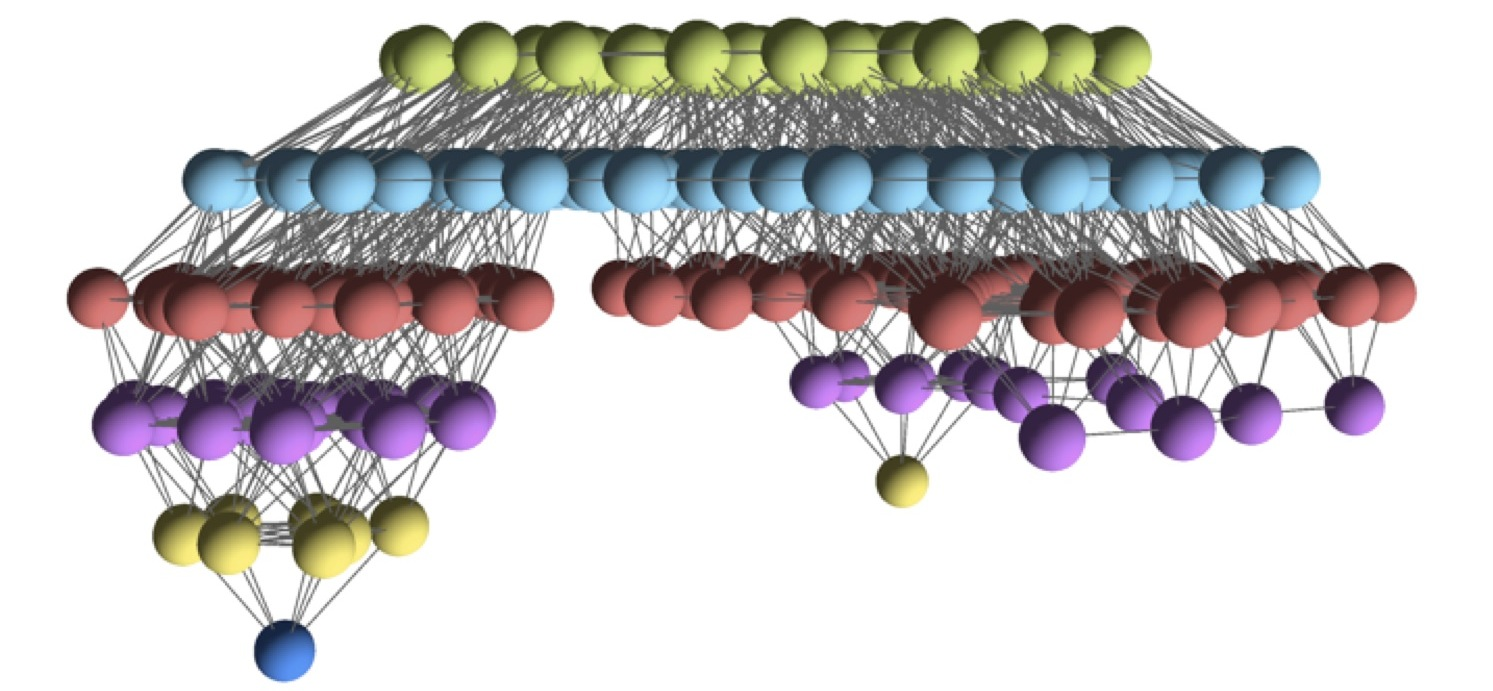
\includegraphics[scale=0.2]{landscape1.jpg}
  \end{center} 
\end{frame}
% \begin{frame}
%  \frametitle{Invarianter}
%  Formål med invarianter
%  \begin{itemize}
%   \item Kan repræsentere en variabel ved en envejsbetingelse
%   \item Kan bruges til at effektivisere lokalsøgning
%  \end{itemize}
%   
% \end{frame}


% \begin{frame}
%  \frametitle{Manglende slides}
%   Mangler at lave en overgang til hvorfor det endte med binær optimering. 
% \end{frame}




% Hvorfor lavet det her? Lave eget system, bygge det på CP med domain reduction. Baserer lokal søgning oven på CP. 
\section{Opbygning af systemet}


%------------------------------------------------	
%\section{Definition af problemer}
\begin{frame}
\frametitle{Binære optimeringsproblemer}
\begin{center}
        $min \left\{\sum\limits_{j=1}^n c_jx_j \; \Big| \; \sum\limits_{j=1}^n a_{ij}x_j \leq b_j \; , \; \; 
\forall i \in 
\{1..m\}\right\}$
\pause
\medskip \\
% \end{center}
% \begin{table}[]
% \begin{center}
% \label{my-label}
\begin{tabular}{llrcrlrl}
Minimize   & z =&$2x_1$        & +  & $x_2$       & + & $x_3$ &          \\
subject to &     &$-x_1$        & + & $2x_2$      &   &       & $\leq 1$  \\
           &     &$x_1$         & + & $x_2$       & + & $x_3$ & $=2$     \\
               
\end{tabular} \\ 
% \end{table}
 $x_1,x_2,x_3 $  $\in$ $\{0,1\}$ 
 \pause
\end{center}
\begin{columns}[T]
    \begin{column}[T]{.5\textwidth}
    \begin{itemize}[<+->]
     \item [--]Mange problemer kan modelleres som binære optimeringsproblemer 
%      \item [--]Mange problemer kan modelleres som binære optimeringsproblemer 
    \end{itemize}
    \end{column}
    
       \begin{column}[T]{.5\textwidth}
           \begin{itemize}[<+->]
     \item [--]Fx: traveling salesman problem, knapsack, vertex cover, ... \newline\newline
    \end{itemize}
       \end{column}
       
\end{columns} 
\onslide<5->{
	  Bliver oprettet i dette system med \textbf{linear}: \medskip \\
	  \footnotesize{\textbf{linear}($int$[]\; coefficients,\; $Variable$[]\; variables,\; $int$\; relation,\; 
 $int$\; bound, \;$int$\; priority)}}

% \begin{align}
%  \text{Minimize }\; &z =  \mathbf{c}^T\mathbf{x} \\ 
%  \text{subject to } \; & \mathbf{A}\mathbf{x} \leq \mathbf{b} \\ 
%  & \mathbf{x} \in \{0,1\}^n
% \end{align} \noindent
  
\end{frame}

%------------------------------------------------

% \begin{frame}
% \frametitle{Eksempel}
% % \begin{align}
% %  \text{Minimize }\; z =  2&x_1 + x_2 + x_3\\ 
% %  \text{subject to } \;  - &x_1 + 2x_2 \leq 1 \\
% %  & x_1 +x_2 + x_3 = 2 \\
% %  & \mathbf{x} \in \{0,1\}^3
% % \end{align} \noindent
% \begin{table}[]
% \begin{center}
% \label{my-label}
% \begin{tabular}{llrcrlrl}
% Minimize   & z = & $2x_1$        & +  & $x_2$       & + & $x_3$ &          \\
% subject to &     & $-x_1$        & + & $2x_2$      &   &       & $\leq 1$  \\
%            &     & $x_1$         & + & $x_2$       & + & $x_3$ & $=2$     
%                
% \end{tabular}
% \end{center}
% $\qquad \qquad $  $x_1,x_2,x_3 $  $\in$ $\{0,1\}$ 
% \end{table}
% En mulig løsning: \\
% \vspace{0.2cm}
% \begin{minipage}{0.47\linewidth}
%  $x_1 = 1$  \\
%  $x_2 = 0$ \\ 
%  $x_3 = 1$ \\
% \end{minipage}
% \begin{minipage}{0.47\linewidth}
% 
%  $z = 2\cdot 1 + 1\cdot 0 + 1\cdot 1  =3$ \\
% \end{minipage}
% \end{frame}
% 
% %------------------------------------------------
% 
% \section{Løsningsmetoder}
% \begin{frame}
% \frametitle{Helttals programmering}
% \begin{itemize}[<+->]  
% \item Simplex metode.
% \item Ligningsbaseret model.
% \item Kan ikke altid finde en (optimal) løsning inden for rimelig tid.
% \item Gurobi, GLPK, SCIP.
% \end{itemize}
% \begin{center}
% \end{center}
% \end{frame}
% 
% %------------------------------------------------
% 
% \begin{frame}
% \frametitle{Constraint programming}
% \begin{itemize}[<+->]
% \item Bruger søgetræer til at finde en løsning.
% \item Mere naturlig formulering af problemer.
% \item bl.a. Gecode, prolog.
% \end{itemize}
% % \begin{center}
% \end{frame}
% 
% \begin{frame}
% \frametitle{Lokal søgning}
% \begin{itemize}[<+->]
% \item Ændre få variable ad gangen og ser beregner effekten.
% \item Kan undersøge mange mulige løsninger.
% \item Kan ikke garantere optimalitet.
% \item Ofte implementeret til specifikke problemer.
% \end{itemize}
% % \begin{center}
% \end{frame}

% 
% \begin{frame}
% \frametitle{Constraint programming med lokalsøgning}
% \begin{itemize}[<+->]
% \item Formulering af problem som i Constraint programming. 
% \item Genanvendelse af algoritmer.
% \item Giver mulighed for at fokusere på modellering.
% \item Solver fx Comet og OscaR.
% \end{itemize}
% % \begin{center}
% \end{frame}
% 
% 
% \begin{frame}
% \frametitle{Hvad er gjort i det her projekt}
% \begin{itemize}[<+->] 
% \item Kombinere Gecode og lokal søgning.
% \item Undersøger effekten af Gecode. 
% \item Tester brugen af invarianter. 
% \item Introducerer en ny evalueringsmetode.
% \end{itemize}
% \end{frame}


%------------------------------------------------
% \section{Finding a maximal matching}
%------------------------------------------------


%------------------------------------------------

% \begin{frame}
% \frametitle{Overblik}
% \begin{itemize}[<+->] 
% \item Objekter, en kasse med værktøj og information. 
% \item Brugerflade og to delt system. 
% \end{itemize}
% Her er et flot billed af formulering -> GPSolver -> GecodeEngine -> LocalSearcEngine. 
% 
% \end{frame}
\begin{frame}
 \frametitle{Før lokalsøgning kan startes}
%  \begin{columns}[T]
%     \begin{column}[T]{.5\textwidth}
Find en startløsning:
\begin{itemize}
\item Opret variable og begrænsninger \pause 
\item Domæne reducering lavet af Gecode \pause 
\item Oprettelse af søgningsstrategi til Gecode \pause 
\item Find en gyldig løsning \pause 
\begin{itemize}
 \item[--] til 100 \% af betingelserne
 \item[--] til 50 \% af betingelserne
 \item[--] til 25 \% af betingelserne
 \item[--] Tilfældig tildeling af værdi til variable inden for deres domæne
\end{itemize}
\end{itemize}
% \end{column}
% \begin{column}[T]{.5\textwidth}
% \onslide<10->
\end{frame}
\begin{frame}
Behandling af betingelser: \pause
 \begin{enumerate}[<+->]
\item Invarianter: Variable defineret af betingelser
\item Graf over afhængighed mellem variable og invarianter
\item Auxiliary invarianter: Betingelser behandlet som invarianter
\item Topologisk sortering af invarianter.
\end{enumerate}

% \end{column}

% \end{columns}
\end{frame}

% 
% \begin{frame}
% \frametitle{}
% 
% \end{frame}

%------------------------------------------------
% \begin{frame}
% \frametitle{Forberedelse til lokalsøgning}
% \begin{itemize}[<+->]
% \item Definer variable ud fra betingelser hvis muligt
% \item Graf over afhængighed
% \item Betingelser lavet som invarianter
% \item Ordning af invarianter.
% \end{itemize}
% \end{frame}

%------------------------------------------------

% \begin{frame}
% \frametitle{Uafhængige variable gjort afhængige}
% \begin{itemize}[<+->]
% \item Færre mulige løsninger der skal undersøges.
% \item Bruger lidt mere tid på at evaluere en løsning.
% \item $x_1 +x_2 -x_3 = 1$.
% \item $x_3 = x_1 +x_2 -1$.
% \item $x_3$ er gjort afhængig af $x_1$ og $x_2$. 
% \item Fjerner betingelsen da den altid vil være overholdt.
% \end{itemize}
% 
% \end{frame}

%------------------------------------------------


\begin{frame}
\frametitle{(1) Invarianter og afhængighedsgraf}
\begin{itemize}[<+->]
 \item Betingelses bestemt om envejsbetingelse kan laves
 \end{itemize}
\[  x_1 + x_2 -x_3 = 1 \; \Leftrightarrow \; x_3 = x_1 +x_2 -1\]
  \[x_3-x_4+x_5  =1 \; \Leftrightarrow \; x_4 = x_3 + x_5 - 1\]
\onslide<3->
\begin{columns}[T]
 \begin{column}[T]{.1\linewidth}
  \end{column}
 \begin{column}[T]{.1\linewidth}
 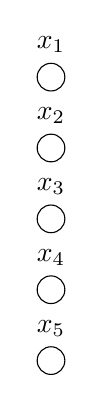
\begin{tikzpicture}[scale=0.9]
        \vertex[label=$x_1$](x1) at (1,4) {};
        \vertex[label=$x_2$](x2) at (1,3) {};
        \vertex[label=$x_3$](x3) at (1,2) {};
        \vertex[label=$x_4$](x4) at (1,1) {};
        \vertex[label=$x_5$](x5) at (1,0) {};
            \end{tikzpicture}
 \end{column}
 \begin{column}[T]{.1\textwidth}
  \onslide<4->
  \vspace{2.3cm}
\Arrow
\end{column}
\begin{column}[T]{0.3\textwidth}
   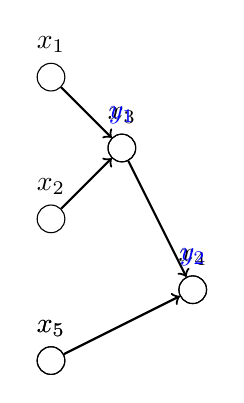
\begin{tikzpicture}[scale=0.9]
          \onslide<4->{\vertex[label=$x_1$](x1) at (0,4) {};}
           \onslide<4->{\vertex[label=$x_2$](x2) at (0,2) {};}
           \onslide<5->{\vertex[label=$x_5$](x5) at (0,0) {};}
           \onslide<4-5>{\vertex[label=$x_3$](i1) at (1,3) {};}
           \onslide<5>{\vertex[label=$x_4$](i2) at (2,1) {};}
      \tikzset{EdgeStyle/.style={->}}
           \onslide<4->{\Edge(x1)(i1)}
           \onslide<4->{\Edge(x2)(i1)}
           \onslide<5->{\Edge(i1)(i2)}
           \onslide<5->{\Edge(x5)(i2)}
          %        \begin{tikzpicture}[scale=0.7]
%             \onslide<5>{\vertex[label=$x_1$](x1) at (0,4) {};}
%              \onslide<5>{\vertex[label=$x_2$](x2) at (0,2) {};}
             \onslide<5->{\vertex[label=$x_5$](x5) at (0,0) {};}
             \onslide<6->{\vertex[label= \color{blue}$y_1$](i1) at (1,3) {};}
             \onslide<6->{\vertex[label= \color{blue}$y_2$](i2) at (2,1) {};}
        \tikzset{EdgeStyle/.style={->}}
%              \onslide<5-6>{\Edge(x1)(i1)}
%              \onslide<5-6>{\Edge(x2)(i1)}
%              \onslide<6>{\Edge(i1)(i2)}
%              \onslide<6>{\Edge(x5)(i2)}
      \end{tikzpicture}
\end{column}
\begin{column}[T]{.55\textwidth}
\pause \pause
\pause
\pause

\begin{itemize}[<+->]
\item $x_3$ er gjort afhængig af $x_1$ og $x_2$
\item $x_4$ indirekte afhængig af $x_1$ og $x_2$
\item Variable valgt efter antal udgående kanter og antallet af betingelser den optræder i
\item \alert{Færre mulige løsninger der skal undersøges}
\item Bruger lidt mere tid på at evaluere en løsning
\end{itemize}
\end{column}


 
\end{columns}

%  \begin{minipage}{0.1\linewidth}
% % \begin{figure}
%      \centering
%      \begin{tikzpicture}[scale=0.9]
%         \vertex[label=$x_1$](x1) at (0,4) {};
%         \vertex[label=$x_2$](x2) at (0,3) {};
%         \vertex[label=$x_3$](x3) at (0,2) {};
%         \vertex[label=$x_4$](x4) at (0,1) {};
%         \vertex[label=$x_5$](x5) at (0,0) {};
%             \end{tikzpicture}
%  \end{minipage}
%  \onslide<4-6>
% \Arrow
% %   \onslide<4-5>
% % \visible<4-5>
%     \begin{minipage}{0.5\linewidth}
%     \centering
%   \begin{tikzpicture}[scale=0.7]
%           \onslide<4-6>{\vertex[label=$x_1$](x1) at (0,4) {};}
%            \onslide<4-6>{\vertex[label=$x_2$](x2) at (0,2) {};}
%            \onslide<5-6>{\vertex[label=$x_5$](x5) at (0,0) {};}
%            \onslide<4-5>{\vertex[label=$x_3$](i1) at (1,3) {};}
%            \onslide<5>{\vertex[label=$x_4$](i2) at (2,1) {};}
%       \tikzset{EdgeStyle/.style={->}}
%            \onslide<4-6>{\Edge(x1)(i1)}
%            \onslide<4-6>{\Edge(x2)(i1)}
%            \onslide<5-6>{\Edge(i1)(i2)}
%            \onslide<5-6>{\Edge(x5)(i2)}
%           %        \begin{tikzpicture}[scale=0.7]
% %             \onslide<5>{\vertex[label=$x_1$](x1) at (0,4) {};}
% %              \onslide<5>{\vertex[label=$x_2$](x2) at (0,2) {};}
%              \onslide<5-6>{\vertex[label=$x_5$](x5) at (0,0) {};}
%              \onslide<6>{\vertex[label= \color{blue}$y_1$](i1) at (1,3) {};}
%              \onslide<6>{\vertex[label= \color{blue}$y_2$](i2) at (2,1) {};}
%         \tikzset{EdgeStyle/.style={->}}
% %              \onslide<5-6>{\Edge(x1)(i1)}
% %              \onslide<5-6>{\Edge(x2)(i1)}
% %              \onslide<6>{\Edge(i1)(i2)}
% %              \onslide<6>{\Edge(x5)(i2)}
%       \end{tikzpicture}
%    \end{minipage}
\end{frame}

%------------------------------------------------
\begin{frame}
\frametitle{(2) Kredse i grafen}
\pause
\begin{columns}[T]
\begin{column}[T]{.1\linewidth}
 
\end{column}
  
\begin{column}[T]{.4\linewidth}  
 \only<1-14>{
 $y_1 = x_1 - y_3$ \\
   $y_2 = y_1 $ \\
 $y_3 = x_2 +y_2-1$ \\
  $x_1,x_2 \in \{0,1\}$ \\ 
  $y_1,y_2,y_3 \in \{0,1\}$  \newline }
  \only<15>{
  $y_1 = x_1 - y_3$ \\
 {\color{red} $y_2 = y_1 $} \\
  $y_3 = x_2 + {\color{red}y_2} - 1$  \\
  $x_1,x_2 \in \{0,1\}$ \\ 
  $y_1, {\color{red}y_2},y_3 \in \{0,1\}$  \newline }
  \only<16->{
   $y_1 = x_1 - y_3$ \\
  $x_3-y_1 = 0$ \\
  $y_3 = x_2 +x_3-1$  \\
  $x_1,x_2,x_3 \in \{0,1\}$ \\ 
  $y_1,y_3 \in \{0,1\}$  \newline}
   \begingroup
%     \fontsize{9pt}{12pt}\selectfont
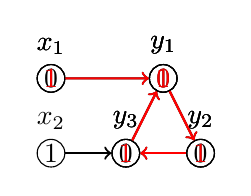
\begin{tikzpicture}[scale=1.9]
        \onslide<3>{\vertex[label=$x_1$](x1) at (0,0.5) {0};}
        \onslide<5->{\vertex[label=$x_1$](x1) at (0,0.5) {1};}
        \onslide<3->{\vertex[label=$x_2$](x2) at (0,0) {1};}
        \onslide<3-4,9->{\vertex[label=$y_1$](y1) at (0.75,0.5) {0};}
        \onslide<6-7>{\vertex[label=$y_1$](y1) at (0.75,0.5) {1};}
        \onslide<3-5>{\vertex[label=$y_2$](y2) at (1,0) {0};}
        \onslide<7->{\vertex[label=$y_2$](y2) at (1,0) {1};}
        \onslide<3-6>{\vertex[label=$y_3$](y3) at (0.5,0) {0};}
        \onslide<8->{\vertex[label=$y_3$](y3) at (0.5,0) {1};}
        \onslide<4>{\vertex[label=$x_1$](x1) at (0,0.5) {\color{red}1};}
        \onslide<5>{\vertex[label=$y_1$](y1) at (0.75,0.5) {\color{red}1};}
        \onslide<8>{\vertex[label=$y_1$](y1) at (0.75,0.5) {\color{red}0};}
        \onslide<6>{\vertex[label=$y_2$](y2) at (1,0) {\color{red}1};}
        \onslide<7>{\vertex[label=$y_3$](y3) at (0.5,0) {\color{red}1};}
        \tikzset{EdgeStyle/.style={->}}
             \onslide<3,5->{\Edge(x1)(y1)}
             \onslide<3-4,6->{\Edge(y1)(y2)}
             \onslide<3-5,7->{\Edge(y2)(y3)}
             \onslide<3-6,8->{\Edge(y3)(y1)}
             \onslide<3->{\Edge(x2)(y3)}
             %
             \onslide<4>{\Edge[style={color=red}](x1)(y1)}
             \onslide<5,8>{\Edge[style={color=red}](y1)(y2)}
             \onslide<6>{\Edge[style={color=red}](y2)(y3)}
             \onslide<7>{\Edge[style={color=red}](y3)(y1)}
             %\onslide<3-7>{\Edge[style={color=red}](x2)(y3)}
      \end{tikzpicture}
      \endgroup
      \\
  \onslide<16->    
    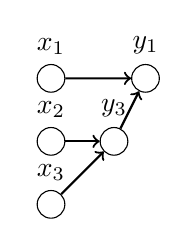
\begin{tikzpicture}[scale=0.8]
 \onslide<2->{\vertex[label=$x_1$](x1) at (0,1) {};}
         \onslide<2->{\vertex[label=$x_2$](x2) at (0,0) {};}
         \onslide<2->{\vertex[label=$x_3$](x3) at (0,-1) {};}
         \onslide<2->{\vertex[label=$y_1$](y1) at (1.5,1) {};}
%         \onslide<>{\vertex[label=$y_1$](y1) at (1,1) {1};}
%         \onslide<2-3>{\vertex[label=$y_2$](y2) at (2,1) {};}
%         \onslide<7-8>{\vertex[label=$y_2$](y2) at (2,1) {1};}
        \onslide<2->{\vertex[label=$y_3$](y3) at (1,0) {};}
        \tikzset{EdgeStyle/.style={->}}
              \onslide<2->{\Edge(x1)(y1)}
              \onslide<2->{\Edge(x3)(y3)}
%              \onslide<2-3>{\Edge(y2)(y3)}
              \onslide<2->{\Edge(y3)(y1)}
             \onslide<2->{\Edge(x2)(y3)}
  \end{tikzpicture}  
  
\end{column}
 \begin{column}[T]{.6\linewidth}  
\pause\pause\pause\pause\pause\pause\pause
 Identificering af kredse:
   \begin{itemize}[<+->]
  \item Dybde først lignende algoritme, af Tarjan $O(V+E)$ 
  \begin{itemize}
  \item [--] Finder stærke sammenhængskomponenter (SCC)
  \item [--] Fjerne en invariant $\rightarrow$ genskaber en variable fra hver SCC
  \item [--] Vælger invariant efter antal indgående kanter
    \end{itemize}
  \item Gentages indtil ingen stærke sammenhængskomponenter er fundet
  \item Balance mellem tid og effekt
%    \item Genindfører variablen $x_3$ og betingelsen.
%    \item $ y_2 = y_1 \Leftrightarrow y_1 -x_3  =0$.
  \end{itemize}

 \end{column}
\end{columns}
\end{frame}
%-------------------------------------------------------
%  \begin{frame}
%  \frametitle{Identificering af kredse}
%  \begin{itemize}[<+->]
%   \item Dybde først lignende algoritme, af Tarjan. 
%   \item Finder stærke sammenhængskomponenter (SCC). 
%   \item Genopretter en betingelse og variable fra hver SCC.
%   \item Gentager indtil ingen stærke sammenhængskomponenter er fundet. 
% \end{itemize}
%     \begin{tikzpicture}[scale=1.7]
%  \onslide<2-3>{\vertex[label=$x_1$](x1) at (0,1) {};}
%          \onslide<2-3>{\vertex[label=$x_2$](x2) at (0,0) {};}
%          \onslide<2-3>{\vertex[label=$x_3$](x3) at (0,-1) {};}
%          \onslide<2-3>{\vertex[label=$y_1$](y1) at (1.5,1) {};}
% %         \onslide<>{\vertex[label=$y_1$](y1) at (1,1) {1};}
% %         \onslide<2-3>{\vertex[label=$y_2$](y2) at (2,1) {};}
% %         \onslide<7-8>{\vertex[label=$y_2$](y2) at (2,1) {1};}
%         \onslide<2-3>{\vertex[label=$y_3$](y3) at (1,0) {};}
%         \tikzset{EdgeStyle/.style={->}}
%               \onslide<2-3>{\Edge(x1)(y1)}
%               \onslide<2-3>{\Edge(x3)(y3)}
% %              \onslide<2-3>{\Edge(y2)(y3)}
%               \onslide<2-3>{\Edge(y3)(y1)}
%              \onslide<2-3>{\Edge(x2)(y3)}
%   \end{tikzpicture}  
%   
%   \onslide<3>
%   \begin{itemize}[<+->]
%    \item Genindfører variablen $x_3$ og betingelsen.
%    \item $ y_2 = y_1 \Leftrightarrow y_1 -x_3  =0$.
%   \end{itemize}
% 
% 
% \end{frame}


%-------------------------------------------------------
%  \begin{frame}
%  \frametitle{Identificering af kredse}
%  \begin{minipage}{0.4\linewidth}
%   \begin{tikzpicture}[scale=1.7]
% %  \onslide<3>{\vertex[label=$x_1$](x1) at (0,1) {0};}
%         \onslide<1-3>{\vertex[label=$x_1$](x1) at (0,1) {};}
%          \onslide<1-3>{\vertex[label=$x_2$](x2) at (0,0) {};}
%         \onslide<1-3>{\vertex[label=$y_1$](y1) at (1.5,1) {};}
% %         \onslide<>{\vertex[label=$y_1$](y1) at (1,1) {1};}
%         \onslide<1-3>{\vertex[label=$y_2$](y2) at (2,0) {};}
% %         \onslide<7-8>{\vertex[label=$y_2$](y2) at (2,1) {1};}
%         \onslide<1-3>{\vertex[label=$y_3$](y3) at (1,0) {};}
%         \tikzset{EdgeStyle/.style={->}}
%              \onslide<1-3>{\Edge(x1)(y1)}
%              \onslide<1-3>{\Edge(y1)(y2)}
%              \onslide<1-3>{\Edge(y2)(y3)}
%              \onslide<1-3>{\Edge(y3)(y1)}
%              \onslide<1-3>{\Edge(x2)(y3)}
%   \end{tikzpicture}
%   \end{minipage}
%   \onslide<2-3>
%   \Arrow \hfill
%      \begin{minipage}{0.45\linewidth}
%     \begin{tikzpicture}[scale=1.7]
%  \onslide<2-3>{\vertex[label=$x_1$](x1) at (0,1) {};}
%          \onslide<2-3>{\vertex[label=$x_2$](x2) at (0,0) {};}
%          \onslide<2-3>{\vertex[label=$x_3$](x3) at (0,-1) {};}
%          \onslide<2-3>{\vertex[label=$y_1$](y1) at (1.5,1) {};}
% %         \onslide<>{\vertex[label=$y_1$](y1) at (1,1) {1};}
% %         \onslide<2-3>{\vertex[label=$y_2$](y2) at (2,1) {};}
% %         \onslide<7-8>{\vertex[label=$y_2$](y2) at (2,1) {1};}
%         \onslide<2-3>{\vertex[label=$y_3$](y3) at (1,0) {};}
%         \tikzset{EdgeStyle/.style={->}}
%               \onslide<2-3>{\Edge(x1)(y1)}
%               \onslide<2-3>{\Edge(x3)(y3)}
% %              \onslide<2-3>{\Edge(y2)(y3)}
%               \onslide<2-3>{\Edge(y3)(y1)}
%              \onslide<2-3>{\Edge(x2)(y3)}
%   \end{tikzpicture}  
%   \end{minipage}
%   
%   \onslide<3>
%   \begin{itemize}[<+->]
%    \item Genindfører variablen $x_3$ og betingelsen.
%    \item $ y_2 = y_1 \Leftrightarrow y_1 -x_3  =0$.
%   \end{itemize}
% 
% \end{frame}

%------------------------------------------------
% \begin{frame}
% \frametitle{Forberedelse til lokalsøgning}
% \begin{itemize}
% \item Definer variable ud fra betingelser hvis muligt.
% \item Graf over afhængighed.
% \item \textbf{Betingelser lavet som invarianter.}
% \item Ordning af invarianter.
% \end{itemize}
% \end{frame}

%------------------------------------------------
 \begin{frame}
 \frametitle{(3) Yderligere invarianter}
 \begin{columns}[T]
\begin{column}[T]{0.55\linewidth} 
 For en \textbf{linear} betingelsen: 
  \begin{itemize}[<+->]
  \item Summering af venstresiden: $\;\underbrace{x_1 + 2x_2 -x_3}_{w_1} \leq 2$
  \item Overtrædelse af betingelsen: $\; \underbrace{w_1 \leq 2}_{w_2}  $\medskip  \\ 
     $w_2 = \begin{cases}
        w_1-2, & \text{if $w_1> 2$}.\\
        0, & \text{otherwise}.
       \end{cases}$
 \end{itemize}
\end{column}
\pause
\begin{column}[T]{0.5\linewidth} 
 \begin{itemize}[<+->]
  \item \alert{Betingelser som ikke er brugt til at definere variable }
  \item Betingelses specifik oprettelse af invarianter
  \item Tilføj invarianter til grafen
  \item Invarianter til summering af overtrædelse betingelser
\end{itemize}

\end{column}
\end{columns}
 \end{frame}


%------------------------------------------------

% \begin{frame}
%  \frametitle{Invarianter for linear}
%  \begin{itemize}[<+->]
%   \item Summering af venstresiden: $\;\underbrace{x_1 + 2x_2 -x_3}_{y_1} \leq 2$
%   \item Overtrædelse af betingelsen: $\; \underbrace{y_1 \leq 2}_{y_2} \;, $
% \end{itemize}
%      $\qquad \qquad y_2 = \begin{cases}
%         y_1-2, & \text{if $y_1> 2$}.\\
%         0, & \text{otherwise}.
%        \end{cases}$
% \end{frame}
%-----------------------------------------------------
\begin{frame}
 \frametitle{Endelige graf}
   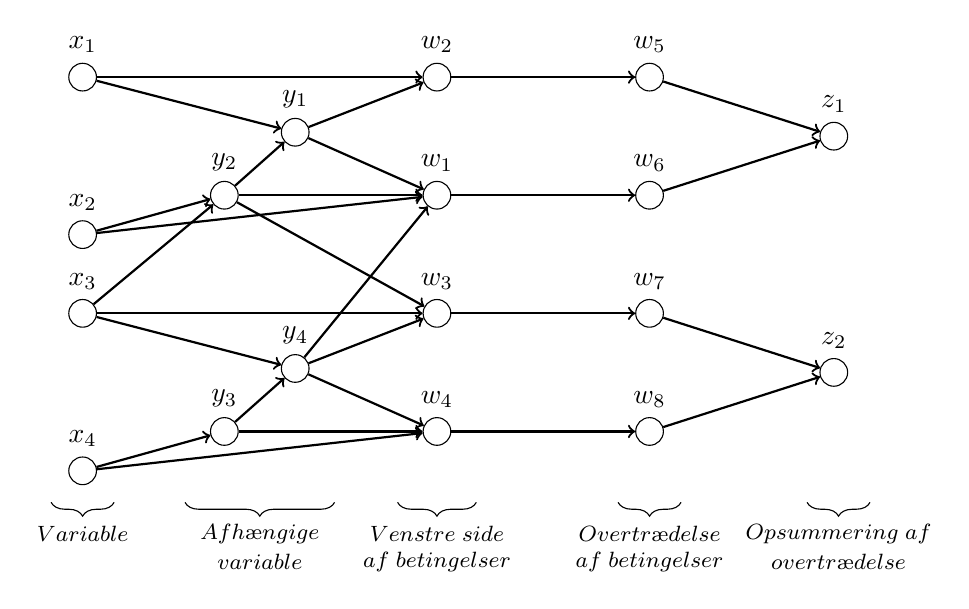
\begin{tikzpicture}[x=1.8cm,y=1cm] %[scale=1]
   \draw [decorate,decoration={brace,amplitude=5pt},xshift=-0pt,yshift=-0pt,rotate=270]
   (0.5,0.4) -- (0.5,-0.4) node [black,midway,yshift=-0.4cm] 
{\footnotesize $Variable$};
\onslide<2-5>{
   \draw [decorate,decoration={brace,amplitude=5pt},xshift=-0pt,yshift=-0pt,rotate=270]
   (0.5,3.2) -- (0.5,1.3) node [black,midway,yshift=-0.4cm] 
{\footnotesize $Afhængige$};
   \draw [decorate,decoration={brace,amplitude=5pt},xshift=-0pt,yshift=-0pt,rotate=270]
   (0.7,2.25) -- (0.7,2.25) node [black,midway,yshift=-0.4cm] 
{\footnotesize $variable$};
}
\onslide<3-5>{
   \draw [decorate,decoration={brace,amplitude=5pt},xshift=-0pt,yshift=-0pt,rotate=270]
   (0.5,5) -- (0.5,4) node [black,midway,yshift=-0.4cm] 
{\footnotesize $Venstre\; side$};
   \draw [decorate,decoration={brace,amplitude=5pt},xshift=-0pt,yshift=-0pt,rotate=270]
   (0.7,4.5) -- (0.7,4.5) node [black,midway,yshift=-0.4cm] 
   {\footnotesize $af\; betingelser$};
   }
   \onslide<4-5>{
\draw [decorate,decoration={brace,amplitude=5pt},xshift=-0pt,yshift=-0pt,rotate=270]
   (0.5,7.6) -- (0.5,6.8) node [black,midway,yshift=-0.4cm] 
   {\footnotesize $Overtrædelse$};
      \draw [decorate,decoration={brace,amplitude=5pt},xshift=-0pt,yshift=-0pt,rotate=270]
   (0.7,7.2) -- (0.7,7.2) node [black,midway,yshift=-0.4cm] 
   {\footnotesize $af\; betingelser$};
   }
   \onslide<5>{
   \draw [decorate,decoration={brace,amplitude=5pt},xshift=-0pt,yshift=-0pt,rotate=270]
   (0.5,10) -- (0.5,9.2) node [black,midway,yshift=-0.4cm] 
   {\footnotesize $Opsummering\;af$};
   \draw [decorate,decoration={brace,amplitude=5pt},xshift=-0pt,yshift=-0pt,rotate=270]
      (0.7,9.6) -- (0.7,9.6) node [black,midway,yshift=-0.4cm] 
   {\footnotesize $overtrædelse$};
   }
         \onslide<1-5>{\vertex[label=$x_3$](x3) at (0,1.5) {};}
          \onslide<1-5>{\vertex[label=$x_4$](x4) at (0,-.5) {};}
         \onslide<2-5>{\vertex[label=$y_4$](y4) at (1.5,0.8) {};}
         \onslide<3-5>{\vertex[label=$w_4$](w4) at (2.5,0) {};}
         \onslide<2-5>{\vertex[label=$y_3$](y3) at (1,0) {};}
         \onslide<3-5>{\vertex[label=$w_3$](w3) at (2.5,1.5) {};}
         \onslide<4-5>{\vertex[label=$w_8$](w8) at (4,0) {};}
         \onslide<4-5>{\vertex[label=$w_7$](w7) at (4,1.5) {};}
         \onslide<5>{\vertex[label=$z_2$](z2) at (5.3,0.75) {};}
         \tikzset{EdgeStyle/.style={->}}
              \onslide<2-5>{\Edge(x3)(y4)}
              \onslide<2-5>{\Edge(y3)(y4)}
              \onslide<2-5>{\Edge(x4)(y3)}
              \onslide<3-5>{\Edge(y3)(w4)}
              \onslide<3-5>{\Edge(x3)(w3)}
              \onslide<3-5>{\Edge(y4)(w3)}
              \onslide<3-5>{\Edge(y4)(w4)}
              \onslide<3-5>{\Edge(x4)(w4)}
	      \onslide<4-5>{\Edge(w3)(w7)}
              \onslide<4-5>{\Edge(w4)(w8)}
              \onslide<5>{\Edge(w8)(z2)}
              \onslide<5>{\Edge(w7)(z2)}
              
         \onslide<1-5>{\vertex[label=$x_1$](x1) at (0,4.5) {};}
          \onslide<1-5>{\vertex[label=$x_2$](x2) at (0,2.5) {};}
         \onslide<2-5>{\vertex[label=$y_1$](y1) at (1.5,3.8) {};}
         \onslide<3-5>{\vertex[label=$w_1$](w1) at (2.5,3) {};}
         \onslide<2-5>{\vertex[label=$y_2$](y2) at (1,3) {};}
         \onslide<3-5>{\vertex[label=$w_2$](w2) at (2.5,4.5) {};}
         \onslide<4-5>{\vertex[label=$w_6$](w6) at (4,3) {};}
         \onslide<4-5>{\vertex[label=$w_5$](w5) at (4,4.5) {};}
         \onslide<5>{\vertex[label=$z_1$](z1) at (5.3,3.75) {};}
         \tikzset{EdgeStyle/.style={->}}
              \onslide<2-5>{\Edge(x1)(y1)}
              \onslide<2-5>{\Edge(x2)(y2)}
              \onslide<2-5>{\Edge(y2)(y1)}
              \onslide<3-5>{\Edge(y1)(w1)}
              \onslide<3-5>{\Edge(x1)(w2)}
              \onslide<3-5>{\Edge(y1)(w2)}
              \onslide<3-5>{\Edge(y2)(w1)}
              \onslide<3-5>{\Edge(x2)(w1)}
	      \onslide<4-5>{\Edge(w2)(w5)}
              \onslide<4-5>{\Edge(w1)(w6)}
              \onslide<5>{\Edge(w5)(z1)}
              \onslide<5>{\Edge(w6)(z1)}
              
              \onslide<2-5>{\Edge(x3)(y2)}
              \onslide<3-5>{\Edge(y4)(w1)}
              \onslide<3-5>{\Edge(y2)(w3)}

              
   \end{tikzpicture} \end{frame}


%------------------------------------------------
% \begin{frame}
% \frametitle{Forberedelse til lokalsøgning}
% \begin{itemize}
% \item Definer variable ud fra betingelser hvis muligt.
% \item Graf over afhængighed.
% \item Betingelser omdannet til invarianter.
% \item \textbf{Ordning af invarianter.}
% \end{itemize}
% \end{frame}

%----------------------------------------------------------------------------------------

\begin{frame}
\frametitle{Ordning af invarianter}
 \begin{columns}[T]
\begin{column}[T]{0.5\linewidth} 
\begin{itemize}[<+->]
\item Lav ordning af invarianter til når de skal opdateres
\item \alert{Forhindre flere opdateringer af samme invariant}
\item Ordningen kan laves med dybde først søgning i grafen
\item \alert{Opret en liste for hver uafhængig variable}
\end{itemize}
\end{column}
\onslide<5->
\begin{column}[T]{0.5\linewidth} 
 \begingroup
    \fontsize{9pt}{12pt}\selectfont
  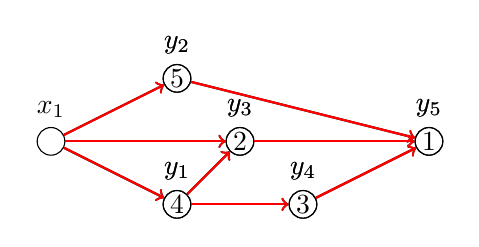
\begin{tikzpicture}[scale=0.8]
        \onslide<5->{\vertex[label=$x_1$](x1) at (0,1) { };}
         \onslide<5-13>{\vertex[label=$y_1$](y1) at (2,0) { };}
        \onslide<5-17>{\vertex[label=$y_2$](y2) at (2,2) { };}
        \onslide<5-9>{\vertex[label=$y_3$](y3) at (3,1) { };}
        \onslide<5-12>{\vertex[label=$y_4$](y4) at (4,0) {};}
        \onslide<5-8>{\vertex[label=$y_5$](y5) at (6,1) {};}
        \tikzset{EdgeStyle/.style={->}}
             \onslide<5,7->{\Edge(x1)(y1)}
             \onslide<5-15,17,19->{\Edge(x1)(y2)}
             \onslide<5-14,16->{\Edge(x1)(y3)}
             \onslide<5-10,12,14->{\Edge(y1)(y4)}
             \onslide<5-6,8-9,11->{\Edge(y1)(y3)}
             \onslide<5-16,18->{\Edge(y2)(y5)}
             \onslide<5-7,10->{\Edge(y3)(y5)}
             \onslide<5-11,13->{\Edge(y4)(y5)}
%         \onslide<13>{\vertex[label=$x_1$](x1') at (0,1) {};}

        \onslide<14->{\vertex[label=$y_1$](y1') at (2,0) {4};}
        \onslide<18->{\vertex[label=$y_2$](y2') at (2,2) {5};}
        \onslide<10->{\vertex[label=$y_3$](y3') at (3,1) {2};}
        \onslide<13->{\vertex[label=$y_4$](y4') at (4,0) {3};}
        \onslide<9->{\vertex[label=$y_5$](y5') at (6,1) {1};}
        \tikzset{EdgeStyle/.style={->}}
             \onslide<6,14>{\Edge[style={color=red}](x1)(y1)}
             \onslide<16,18>{\Edge[style={color=red}](x1)(y2)}
             \onslide<15>{\Edge[style={color=red}](x1)(y3)}
             \onslide<11,13>{\Edge[style={color=red}](y1)(y4)}
             \onslide<7,10>{\Edge[style={color=red}](y1)(y3)}
             \onslide<17>{\Edge[style={color=red}](y2)(y5)}
             \onslide<8-9>{\Edge[style={color=red}](y3)(y5)}
             \onslide<12>{\Edge[style={color=red}](y4)(y5)}
  \end{tikzpicture}
  \onslide<20>
    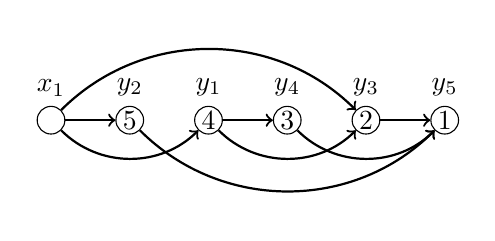
\begin{tikzpicture}[scale=1]
        \vertex[label=$x_1$](x1) at (0,0) {};
        \vertex[label=$y_1$](y1) at (2,0) {4};
        \vertex[label=$y_2$](y2) at (1,0) {5};
        \vertex[label=$y_3$](y3) at (4,0) {2};
        \vertex[label=$y_4$](y4) at (3,0) {3};
        \vertex[label=$y_5$](y5) at (5,0) {1};
        \tikzset{EdgeStyle/.style={->}}
           \Edge[style={bend right = 45}](x1)(y1)
           \Edge[style={bend right = 0}](x1)(y2)
           \Edge[style={bend left = 45}](x1)(y3)
           \Edge[style={bend right = 0}](y1)(y4)
           \Edge[style={bend right = 45}](y1)(y3)
           \Edge[style={bend right = 45}](y2)(y5)
           \Edge[style={bend right = 0}](y3)(y5)
           \Edge[style={bend right = 45}](y4)(y5)
  \end{tikzpicture}
\endgroup
\end{column}
\end{columns}
\end{frame}

%----------------------------------------------------------------------------------------
% 
% \begin{frame}
% \frametitle{Eksempel for en variable}
% \centering
% % \begin{figure}[!t]
% % \centering
% % 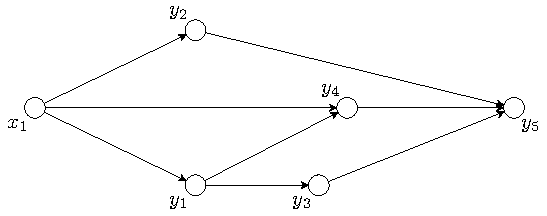
\includegraphics[width=0.6\linewidth]{1.pdf} 
% % % \end{center} 
% % \end{figure}%
% \begingroup
% \begin{center}
%     \fontsize{9pt}{12pt}\selectfont
%   \begin{tikzpicture}[scale=1]
%         \onslide<1-16>{\vertex[label=$x_1$](x1) at (0,1) { };}
%          \onslide<1-9>{\vertex[label=$y_1$](y1) at (2,0) { };}
%         \onslide<1-13>{\vertex[label=$y_2$](y2) at (2,2) { };}
%         \onslide<1-5>{\vertex[label=$y_3$](y3) at (3,1) { };}
%         \onslide<1-8>{\vertex[label=$y_4$](y4) at (4,0) {};}
%         \onslide<1-4>{\vertex[label=$y_5$](y5) at (6,1) {};}
%         \tikzset{EdgeStyle/.style={->}}
%              \onslide<1,3-16>{\Edge(x1)(y1)}
%              \onslide<1-11,13,15,16>{\Edge(x1)(y2)}
%              \onslide<1-10,12-16>{\Edge(x1)(y3)}
%              \onslide<1-6,8,10-16>{\Edge(y1)(y4)}
%              \onslide<1-2,4,5,7-16>{\Edge(y1)(y3)}
%              \onslide<1-12,14-16>{\Edge(y2)(y5)}
%              \onslide<1-3,6-16>{\Edge(y3)(y5)}
%              \onslide<1-7,9-16>{\Edge(y4)(y5)}
% %         \onslide<13>{\vertex[label=$x_1$](x1') at (0,1) {};}
% 
%         \onslide<10-16>{\vertex[label=$y_1$](y1') at (2,0) {4};}
%         \onslide<14-16>{\vertex[label=$y_2$](y2') at (2,2) {5};}
%         \onslide<6-16>{\vertex[label=$y_3$](y3') at (3,1) {2};}
%         \onslide<9-16>{\vertex[label=$y_4$](y4') at (4,0) {3};}
%         \onslide<5-16>{\vertex[label=$y_5$](y5') at (6,1) {1};}
%         \tikzset{EdgeStyle/.style={->}}
%              \onslide<2,10>{\Edge[style={color=red}](x1)(y1)}
%              \onslide<12,14>{\Edge[style={color=red}](x1)(y2)}
%              \onslide<11>{\Edge[style={color=red}](x1)(y3)}
%              \onslide<7,9>{\Edge[style={color=red}](y1)(y4)}
%              \onslide<3,6>{\Edge[style={color=red}](y1)(y3)}
%              \onslide<13>{\Edge[style={color=red}](y2)(y5)}
%              \onslide<4,5>{\Edge[style={color=red}](y3)(y5)}
%              \onslide<8>{\Edge[style={color=red}](y4)(y5)}
%   \end{tikzpicture}
%   \onslide<16>
%     \begin{tikzpicture}[scale=1.2]
%         \vertex[label=$x_1$](x1) at (0,0) {};
%         \vertex[label=$y_1$](y1) at (2,0) {4};
%         \vertex[label=$y_2$](y2) at (1,0) {5};
%         \vertex[label=$y_3$](y3) at (4,0) {2};
%         \vertex[label=$y_4$](y4) at (3,0) {3};
%         \vertex[label=$y_5$](y5) at (5,0) {1};
%         \tikzset{EdgeStyle/.style={->}}
%            \Edge[style={bend right = 45}](x1)(y1)
%            \Edge[style={bend right = 0}](x1)(y2)
%            \Edge[style={bend left = 45}](x1)(y3)
%            \Edge[style={bend right = 0}](y1)(y4)
%            \Edge[style={bend right = 45}](y1)(y3)
%            \Edge[style={bend right = 45}](y2)(y5)
%            \Edge[style={bend right = 0}](y3)(y5)
%            \Edge[style={bend right = 45}](y4)(y5)
%   \end{tikzpicture}
%   \end{center}
% 
% \endgroup
% \end{frame}
% 
% 
\section{Lokalsøgningsalgoritmer}
\begin{frame}
 \frametitle{Basis for algoritmerne}
 \begin{columns}[T]
  \begin{column}[T]{0.5\linewidth}
  \centering
  Fra universitet til stadion \medskip \\
  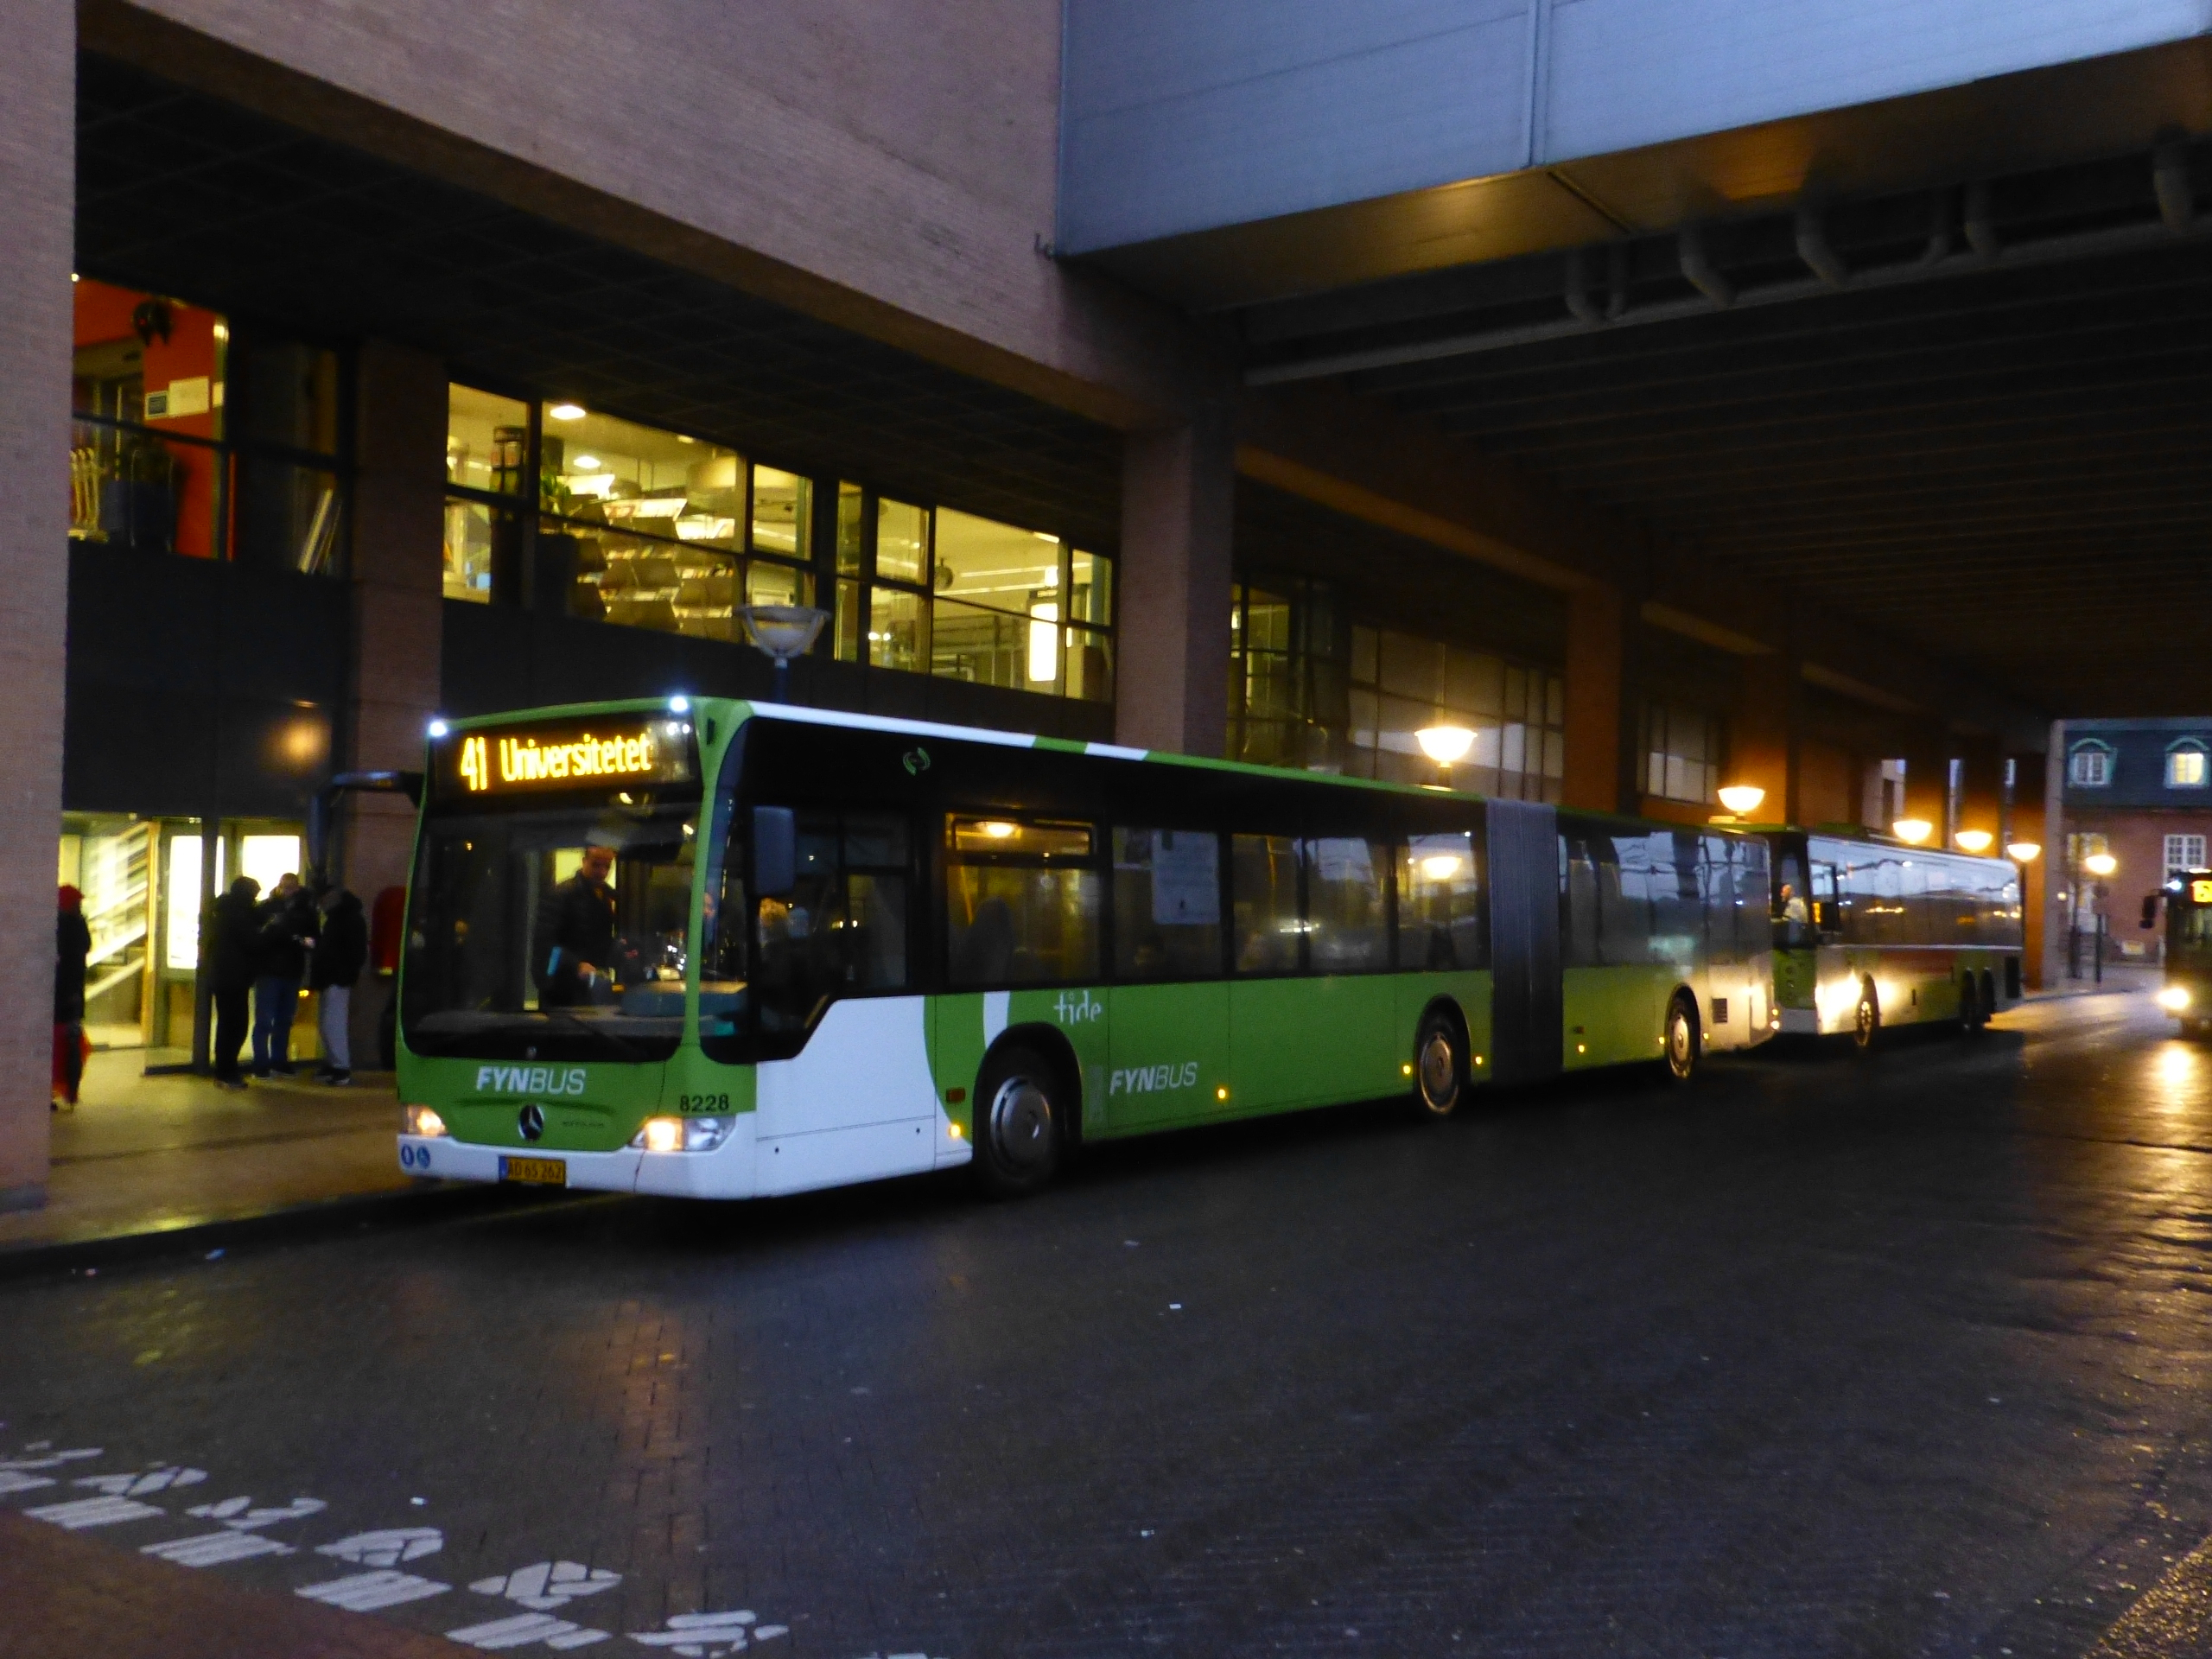
\includegraphics[scale=0.06]{fynbus.JPG}
  \end{column}
\begin{column}[T]{0.5\linewidth}
\begin{itemize}[<+->]
 \item Find den optimale løsning:  \\
 Kan være alt fra trivielt til meget svært 
 \item First improvement: \\ 
 Første der forbedre nuværende situation
 \item Best improvement: \\ 
 Bedste forbedring af nuværende situation
 \item Random walk: \\
 En række tilfældige valg
\end{itemize}
  \end{column}
 \end{columns}

\end{frame}
%----------------------------------------------------------------------------------------
\begin{frame}
 \frametitle{Lokalsøgningsalgoritmer}
\begin{columns}[T]
\begin{column}[T]{0.4\linewidth}
  Bruger kun 1-flip lokalsøgning \pause \medskip \\ 
  Forkortelser: 
 \begin{itemize}
  \item FI: First improvement
  \item TS: Tabu search
  \item CN: Conflict only neighborhood
  \item TL: Time limit
  \item RW: Random walk
  \item MC: Minimum conflict heuristic
 \end{itemize}
\end{column}
\pause
\begin{column}[T]{0.5\linewidth}
\only<1-4>{
\resizebox{6cm}{3cm}{
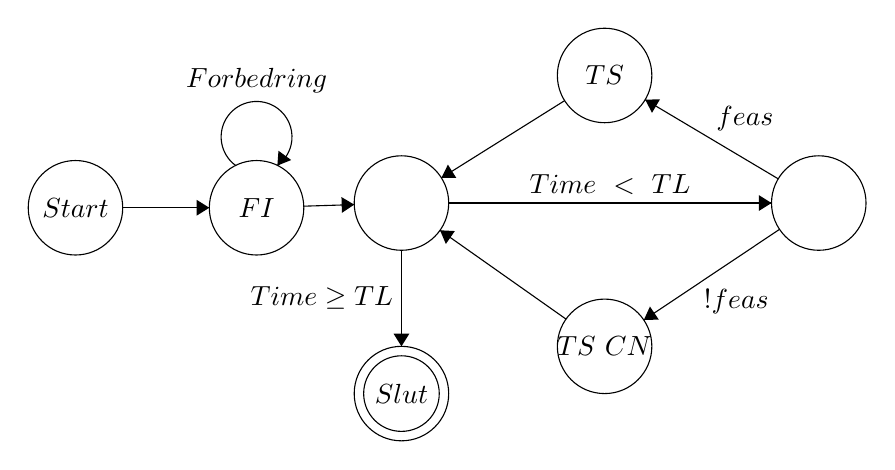
\begin{tikzpicture}[scale=0.2]
\tikzstyle{every node}+=[inner sep=0pt]
\draw [black] (8.9,-32.6) circle (3);
\draw (8.9,-32.6) node {$Start$};
\draw [black] (20.4,-32.6) circle (3);
\draw (20.4,-32.6) node {$FI$};
\draw [black] (42.5,-24.2) circle (3);
\draw (42.5,-24.2) node {$TS$};
\draw [black] (29.6,-32.3) circle (3);
\draw [black] (56.1,-32.3) circle (3);
\draw [black] (42.5,-41.4) circle (3);
\draw (42.5,-41.4) node {$TS$ $CN$};
\draw [black] (29.6,-44.4) circle (3);
\draw (29.6,-44.4) node {$Slut$};
\draw [black] (29.6,-44.4) circle (2.4);
\draw [black] (11.9,-32.6) -- (17.4,-32.6);
\fill [black] (17.4,-32.6) -- (16.6,-32.1) -- (16.6,-33.1);
\draw [black] (19.077,-29.92) arc (234:-54:2.25);
\draw (20.4,-25.35) node [above] {$Forbedring$};
\fill [black] (21.72,-29.92) -- (22.6,-29.57) -- (21.79,-28.98);
\draw [black] (23.4,-32.5) -- (26.6,-32.4);
\fill [black] (26.6,-32.4) -- (25.79,-31.92) -- (25.82,-32.92);
\draw [black] (32.6,-32.3) -- (53.1,-32.3);
\fill [black] (53.1,-32.3) -- (52.3,-31.8) -- (52.3,-32.8);
\draw (42.85,-31.8) node [above] {$Time\mbox{ }<\mbox{ }TL$};
\draw [black] (53.52,-30.76) -- (45.08,-25.74);
\fill [black] (45.08,-25.74) -- (45.51,-26.57) -- (46.02,-25.71);
\draw (51.41,-27.75) node [above] {$feas$};
\draw [black] (39.96,-25.8) -- (32.14,-30.7);
\fill [black] (32.14,-30.7) -- (33.08,-30.7) -- (32.55,-29.86);
\draw [black] (53.61,-33.97) -- (44.99,-39.73);
\fill [black] (44.99,-39.73) -- (45.94,-39.7) -- (45.38,-38.87);
\draw (50.86,-39.35) node [above] {$!feas$};
\draw [black] (40.05,-39.67) -- (32.05,-34.03);
\fill [black] (32.05,-34.03) -- (32.42,-34.9) -- (32.99,-34.08);
\draw [black] (29.6,-35.3) -- (29.6,-41.4);
\fill [black] (29.6,-41.4) -- (30.1,-40.6) -- (29.1,-40.6);
\draw (29.1,-38.35) node [left] {$Time\geq TL$};
\end{tikzpicture}
}}
\only<5>{
\resizebox{6cm}{3cm}{
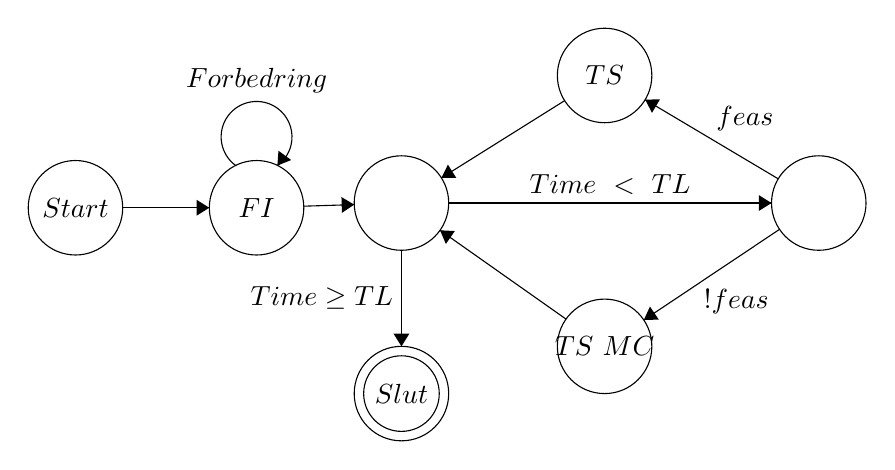
\begin{tikzpicture}[scale=0.2]
\tikzstyle{every node}+=[inner sep=0pt]
\draw [black] (8.9,-32.6) circle (3);
\draw (8.9,-32.6) node {$Start$};
\draw [black] (20.4,-32.6) circle (3);
\draw (20.4,-32.6) node {$FI$};
\draw [black] (42.5,-24.2) circle (3);
\draw (42.5,-24.2) node {$TS$};
\draw [black] (29.6,-32.3) circle (3);
\draw [black] (56.1,-32.3) circle (3);
\draw [black] (42.5,-41.4) circle (3);
\draw (42.5,-41.4) node {$TS$ $MC$};
\draw [black] (29.6,-44.4) circle (3);
\draw (29.6,-44.4) node {$Slut$};
\draw [black] (29.6,-44.4) circle (2.4);
\draw [black] (11.9,-32.6) -- (17.4,-32.6);
\fill [black] (17.4,-32.6) -- (16.6,-32.1) -- (16.6,-33.1);
\draw [black] (19.077,-29.92) arc (234:-54:2.25);
\draw (20.4,-25.35) node [above] {$Forbedring$};
\fill [black] (21.72,-29.92) -- (22.6,-29.57) -- (21.79,-28.98);
\draw [black] (23.4,-32.5) -- (26.6,-32.4);
\fill [black] (26.6,-32.4) -- (25.79,-31.92) -- (25.82,-32.92);
\draw [black] (32.6,-32.3) -- (53.1,-32.3);
\fill [black] (53.1,-32.3) -- (52.3,-31.8) -- (52.3,-32.8);
\draw (42.85,-31.8) node [above] {$Time\mbox{ }<\mbox{ }TL$};
\draw [black] (53.52,-30.76) -- (45.08,-25.74);
\fill [black] (45.08,-25.74) -- (45.51,-26.57) -- (46.02,-25.71);
\draw (51.41,-27.75) node [above] {$feas$};
\draw [black] (39.96,-25.8) -- (32.14,-30.7);
\fill [black] (32.14,-30.7) -- (33.08,-30.7) -- (32.55,-29.86);
\draw [black] (53.61,-33.97) -- (44.99,-39.73);
\fill [black] (44.99,-39.73) -- (45.94,-39.7) -- (45.38,-38.87);
\draw (50.86,-39.35) node [above] {$!feas$};
\draw [black] (40.05,-39.67) -- (32.05,-34.03);
\fill [black] (32.05,-34.03) -- (32.42,-34.9) -- (32.99,-34.08);
\draw [black] (29.6,-35.3) -- (29.6,-41.4);
\fill [black] (29.6,-41.4) -- (30.1,-40.6) -- (29.1,-40.6);
\draw (29.1,-38.35) node [left] {$Time\geq TL$};
\end{tikzpicture}
}
}
\pause
\resizebox{6cm}{2.8cm}{
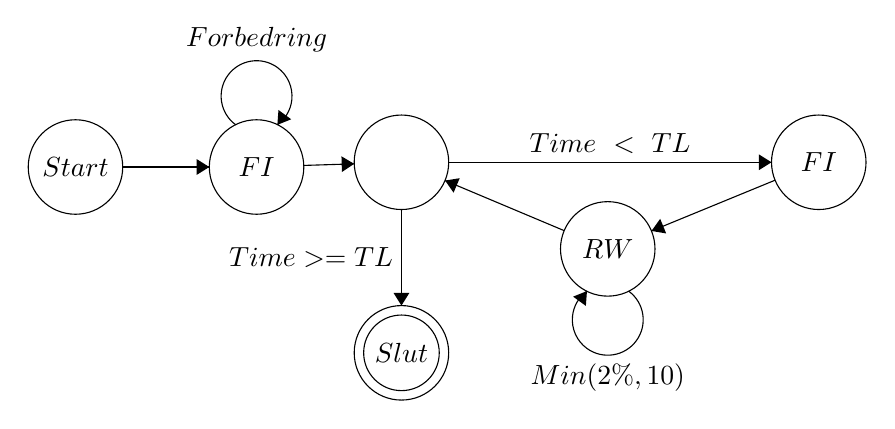
\begin{tikzpicture}[scale=0.2]
\tikzstyle{every node}+=[inner sep=0pt]
\draw [black] (8.9,-32.6) circle (3);
\draw (8.9,-32.6) node {$Start$};
\draw [black] (20.4,-32.6) circle (3);
\draw (20.4,-32.6) node {$FI$};
\draw [black] (29.6,-32.3) circle (3);
\draw [black] (56.1,-32.3) circle (3);
\draw (56.1,-32.3) node {$FI$};
\draw [black] (42.7,-37.8) circle (3);
\draw (42.7,-37.8) node {$RW$};
\draw [black] (29.6,-44.4) circle (3);
\draw (29.6,-44.4) node {$Slut$};
\draw [black] (29.6,-44.4) circle (2.4);
\draw [black] (11.9,-32.6) -- (17.4,-32.6);
\fill [black] (17.4,-32.6) -- (16.6,-32.1) -- (16.6,-33.1);
\draw [black] (19.077,-29.92) arc (234:-54:2.25);
\draw (20.4,-25.35) node [above] {$Forbedring$};
\fill [black] (21.72,-29.92) -- (22.6,-29.57) -- (21.79,-28.98);
\draw [black] (23.4,-32.5) -- (26.6,-32.4);
\fill [black] (26.6,-32.4) -- (25.79,-31.92) -- (25.82,-32.92);
\draw [black] (32.6,-32.3) -- (53.1,-32.3);
\fill [black] (53.1,-32.3) -- (52.3,-31.8) -- (52.3,-32.8);
\draw (42.85,-31.8) node [above] {$Time\mbox{ }<\mbox{ }TL$};
\draw [black] (53.32,-33.44) -- (45.48,-36.66);
\fill [black] (45.48,-36.66) -- (46.41,-36.82) -- (46.03,-35.89);
\draw [black] (39.93,-36.64) -- (32.37,-33.46);
\fill [black] (32.37,-33.46) -- (32.91,-34.23) -- (33.3,-33.31);
\draw [black] (29.6,-35.3) -- (29.6,-41.4);
\fill [black] (29.6,-41.4) -- (30.1,-40.6) -- (29.1,-40.6);
\draw (29.1,-38.35) node [left] {$Time>=TL$};
\draw [black] (44.023,-40.48) arc (54:-234:2.25);
\draw (42.7,-45.05) node [below] {$Min(2\%,10)$};
\fill [black] (41.38,-40.48) -- (40.5,-40.83) -- (41.31,-41.42);
\end{tikzpicture}
}
\end{column}
\end{columns}
\end{frame}




%----------------------------------------------------------------------------------------
\section{Eksperimentel evaluering}
\begin{frame}
\frametitle{Effekten af envejsbetingelser (oneway constraints)}
\begin{figure}[!h]
\centering
\includegraphics[scale=0.3]{../R/oneway}
% \end{center} 
\end{figure}\noindent
\end{frame}


\begin{frame}
\frametitle{Gecode som konstruktions heuristik}
\begin{figure}[!h]
\centering
\includegraphics[scale=0.3]{../R/gecodenols} 
% \end{center} 
\end{figure}\noindent
\end{frame}



\begin{frame}
\frametitle{Gecode som konstruktions heuristik}
\begin{figure}[!h]
\centering
\includegraphics[scale=0.3]{../R/gecodetime}
% \end{center} 
\end{figure}\noindent
\end{frame}

\begin{frame}
\frametitle{Gecode som konstruktions heuristik}
\begin{figure}[!h]
\centering
\includegraphics[scale=0.3]{../R/gecodels}
% \end{center} 
\end{figure}\noindent
\end{frame}



\begin{frame}
\frametitle{Algoritmerne mod hinanden}
\begin{figure}[!h]
\centerline{
\includegraphics[scale=0.3]{../R/algs}}
\end{figure}\noindent
\end{frame}


\begin{frame}
\frametitle{Algoritmerne mod hinanden}
\begin{figure}[!h]
\centerline{
\includegraphics[scale=0.3]{../R/algbox}}
\end{figure}\noindent
\end{frame}

\begin{frame}
\frametitle{Eksempel}
\begin{figure}[!h]
\centerline{
\includegraphics[scale=0.3]{../R/conv1}}
\end{figure}\noindent
\end{frame}

\begin{frame}
\frametitle{Eksempel}
\begin{figure}[!h]
\centerline{
\includegraphics[scale=0.3]{../R/conv2}}
\end{figure}\noindent
\end{frame}
\begin{frame}


\frametitle{Eksempel - alle gyldige}
\begin{figure}[!h]
\centerline{
\includegraphics[scale=0.3]{../R/conv3}}
\end{figure}\noindent
\end{frame}



\section{Sidste kommentarer}
\begin{frame}
 \frametitle{Forbedringer og udvidelser}
 \begin{columns}[T]
  \begin{column}[T]{0.5\linewidth}
    Forbedringer:  \pause
    \begin{itemize}[<+->]
    \item En bedre konstruktionsheuristik hvis Gecode ikke kan bruges
     \item Implementering swap som neighborhood operation
     \item Implementering af simuleret udglødning
     \item Test af flere parametre bl.a. for tabu søgning
     \item Undersøg effekt af opdeling af variable, envejsbetingelser
    \end{itemize}
  \end{column}
%       \pause
      \onslide<7->
\begin{column}[T]{0.5\linewidth}
  Udvidelser: \pause
   \begin{itemize}[<+->]
     \item Tillad ikke heltalskoefficienter 
     \item Behandling af heltalsvariable
     \item Flere typer af betingelser
     \item Flere skift mellem CP og LS
    \end{itemize}
  \end{column}

 \end{columns}

\end{frame}

\begin{frame}
 \frametitle{Konklusion}
    \begin{itemize}[<+->]
     \item Et CBLS system der danner grundlag for udvidelser
     \item Gecode begrænset effekt på Binær programmering
     \item Alle variable behandlet med samme neighborhood operation, giver ingen effekt af envejsbetingelser
     \item 
     \item 
    \end{itemize}
\end{frame}







\end{document}